
\thispagestyle{fancy}
\justifying
\chapter{Untersuchung optisch gepumpter Laserstrukturen auf unterschiedlichen Templates}
\label{chap:offcut}

\section{Einleitung}
Dieses Kapitel widmet sich der Untersuchung zweier Probenreihen von optisch gepumpten Laserstrukturen, die aus Rezepten aus zwei unterschiedlichen Serien stammen. Die beiden Serien unterscheiden sich im wesentlichen dadurch, dass sie mit(Serie 2) und ohne Übergitter(Serie 1) gewachsen wurden. Sie haben alle eine aktive Zone, die sich zusammen setzt aus zwei $5$nm dicken und siliziumdotierten $ Al_{0.8}Ga_{0.3}N$-Barrieren zwischen den drei $2.2$nm dicken $ Al_{0.56}Ga_{0.44}N$ QWs. Die aktive Zone befindet sich zwischen einem $30 \thinspace nm$ dicken $ Al_{0.70}Ga_{0.30}N$ und einem $85 \thinspace nm$ dicken Waveguide als oberste Schicht. Der Wellenleiter hat den Zweck, die optische Mode einzuschließen, daher ist ein hoher Brechungsindexsprung zwischen den Barrieren der aktiven Region und der darüberlegenden Schichten notwendig.
Dieser Block an Schichten bildet die unveränderte Grundlage für alle in diesem Kapitel untersuchten Proben.
\begin{figure}[H]
\centering
\begin{tabular}{ |c|c|c|c|c|c|   }
\hline
\multicolumn{2}{|c|}{Serie 1} & \multicolumn{2}{c|}{Serie 2}  \\
\hline
Name & offcut&  Name & offcut  \\
\hline
A & 0.1$^\circ$m  & A-SL & 0.1$^\circ$m \\
B & 0.1$^\circ$m* & B-SL & 0.1$^\circ$m* \\
C & 0.2$^\circ$m  & C-SL & 0.2$^\circ$m \\
\hline
\end{tabular}
\end{figure}
\noindent 
Die Proben beider Serien mit dem ELO AlN/Saphir Substrat unterscheiden sich untereinander noch vom Fehlschnitt und der Richtung des Fehlschnittes des Substrats. Die gegeben Werte stammen vom Hersteller und sind nur nominelle Werte die sich von den realen unterscheiden können. So haben die mit A gekennzeichneten Proben einen nominellen Fehlschnitt von $\alpha = 0.1\circ \thinspace m$ in die Standard m-Richtung, die mit B gekennzeichneten Proben den selben Fehlschnitt in eine der sechs nicht Standard m-Richtungen und die mit C gekennzeichneten Proben einen Fehlschnitt von $\alpha = 0.2\circ \thinspace m$ in die Standard m-Richtung. 
Die Untersuchung des Einflusses des Fehlschnitt-Winkels des Substrates, ist insofern interessant, da dieser eine entscheidende Rolle beim Wachstum der Heterostrukturen spielt. Er erlaubt es die Wachstumskinetik zu steuern, so dass sich die Schichten in die kristalline Struktur formen wie in Abbildung \ref{fig:offcut} zu sehen ist.
Der Fehlschnitt-Winkel $\alpha$ ist die Winkel-Differenz zwischen Oberflächennormale und der c-Richtung. Für ein $\alpha \leq 0,12 $ wurde gezeigt, dass es zu Stufenfluss kommt und somit zu relativ glatten Oberflächen mit wellenartiger Morphologie und mit $\alpha \geq 0,16 $ in Stufenbündelwachstum mit Makrostufen resultieren kann. Dies ist nicht unwichtig für Laserstrukturen, da glatte Oberflächen optische Streuung an der Oberfläche verringern, sollten aber keinen Effekt auf die IQE haben. Allerdings kann an den Stufenkanten verstärkt Ga eingebaut und somit die Zusammensetzung der aktiven Zone inhomogen werden \cite{zeimeru} \cite{MOGILATENKO2014222} \cite{fmehnke}, was wiederum einen Einfluss auf die IQE durch Lokalisierung haben könnte.
%
\begin{figure}[htb]
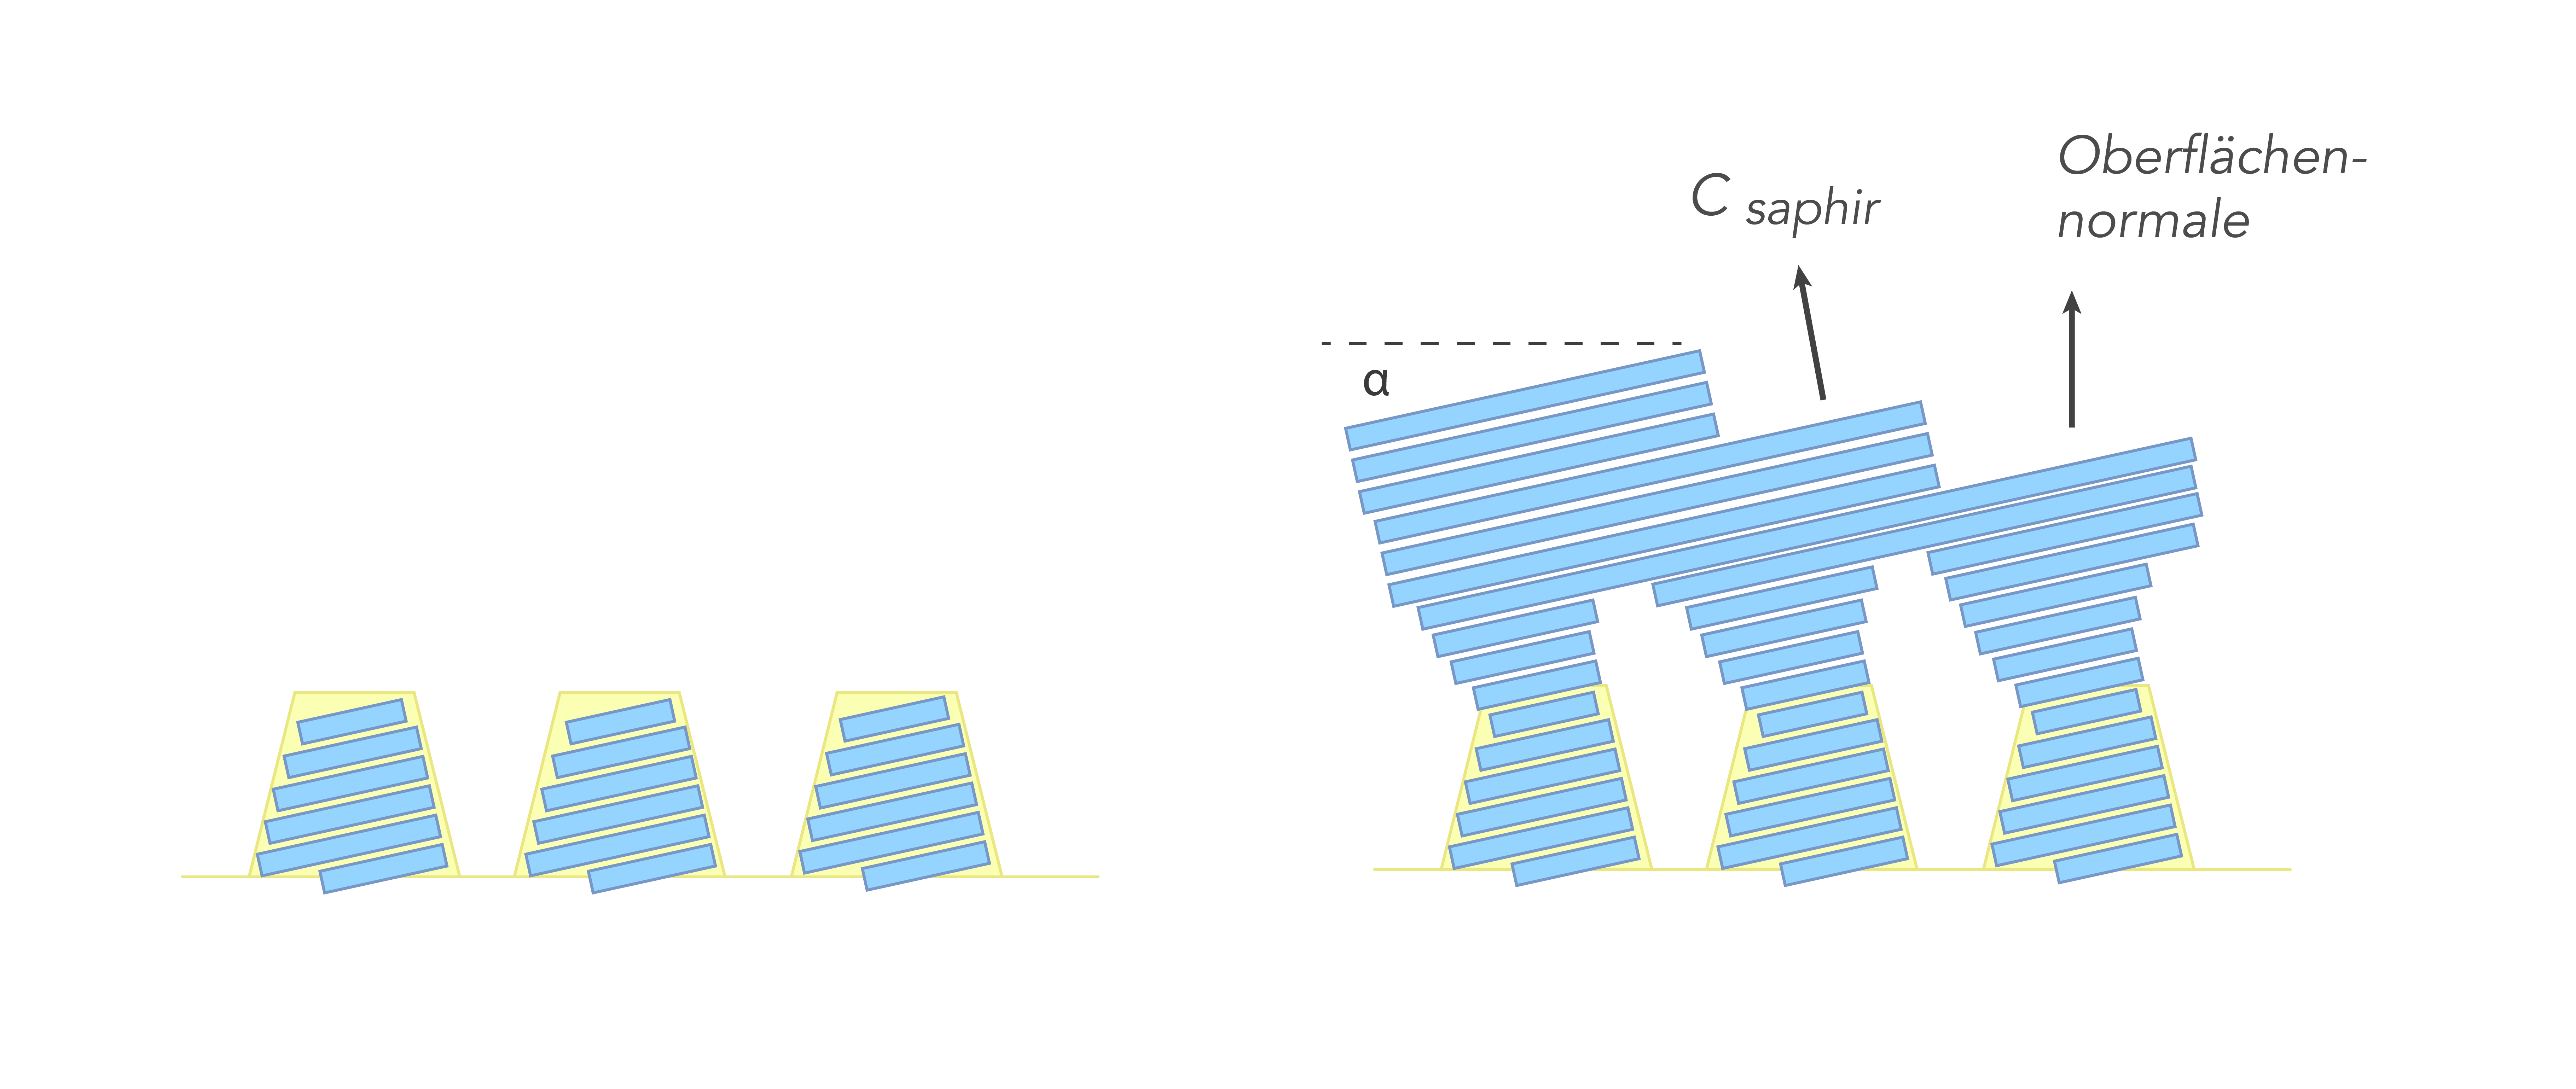
\includegraphics[width=\linewidth]{Bilder/offcut.png}
\caption{Einfluss des Fehlschnitt-Winkels auf das Wachstum bei ELO AlN/Saphir.}
\label{fig:offcut}
\end{figure}
\noindent 
%
Die Makrostufen können zudem zu einer Reduktion der TDD beitragen, die wiederum in der IQE sichtbar ist wie Abbildung \ref{fig:IQEthreadingdisl} zeigt. Bei Proben mit einem geringen Fehlschnitt von $\alpha = 0,12 $ verlaufen die Versetzungen senkrecht zur Kristalloberfläche. Bei Proben mit einem großen Fehlschnitt von $\alpha = 0,16 $ verlaufen die Versetzungen diagonal wie Abbildung \ref{fig:schraubenvers} zeigt. Bei diesen Versetzungen handelt es sich um sogenannten Koaleszenzkorngrenzen die an der Oberfläche als Makrostufen zu erkennen sind \cite{MOGILATENKO2014222}. 
%
\begin{figure}[htb]
  \centering
  \begin{minipage}[t]{0.49\textwidth}
    \centering
    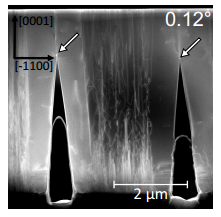
\includegraphics[width=0.6\textwidth]{Bilder/offcutsenkrecht.png}
    \label{}
  \end{minipage}
	\hfill
  \begin{minipage}[t]{0.49\textwidth}
    \centering
    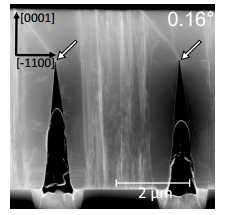
\includegraphics[width=0.6\linewidth]{Bilder/offcutdiagonal.png}
    \label{}
  \end{minipage}
	\caption{Querschnitts-TEM-Aufnahmen mit den sichtbaren senkrecht und diagonal verlaufenden Schraubenversetzungen}
	\label{schraubenvers}
\end{figure}
%
Bei Schichtdicken $ \geq 10 \mu m $ kreuzen diese diagonal verlaufenden Makrostufen die versetzungsreichen Gebiete zwischen den geätzten Gräben im ELO oft genug um diese fast vollständig zu annhilieren \cite{fmehnke}. Solche Dicken sind aber schwierig zu realisieren durch das schwierige Wachstum und der entstehenden Krümmung des Wafers. Bei den hier verwendeten Schichtdicken von $ \geq 1\thinspace \mu m $ ist nur eine teilweise Annihilation und damit eine Defektreduktion von $1\cdot 10^{10} \thinspace cm^{-2}$ auf $5\cdot 10^9 \thinspace cm^{-2}$ zu erwarten \cite{fmehnke}. Weiter beachtet werden muss, dass bei den darauf folgenden Schichten eine Planarisierung stattfinden muss, um eine möglichst ebene aktive Zone zu haben. 

\section{UVC-Laser Strukturen auf ELO ohne Übergitter}
%
\begin{figure}[h]
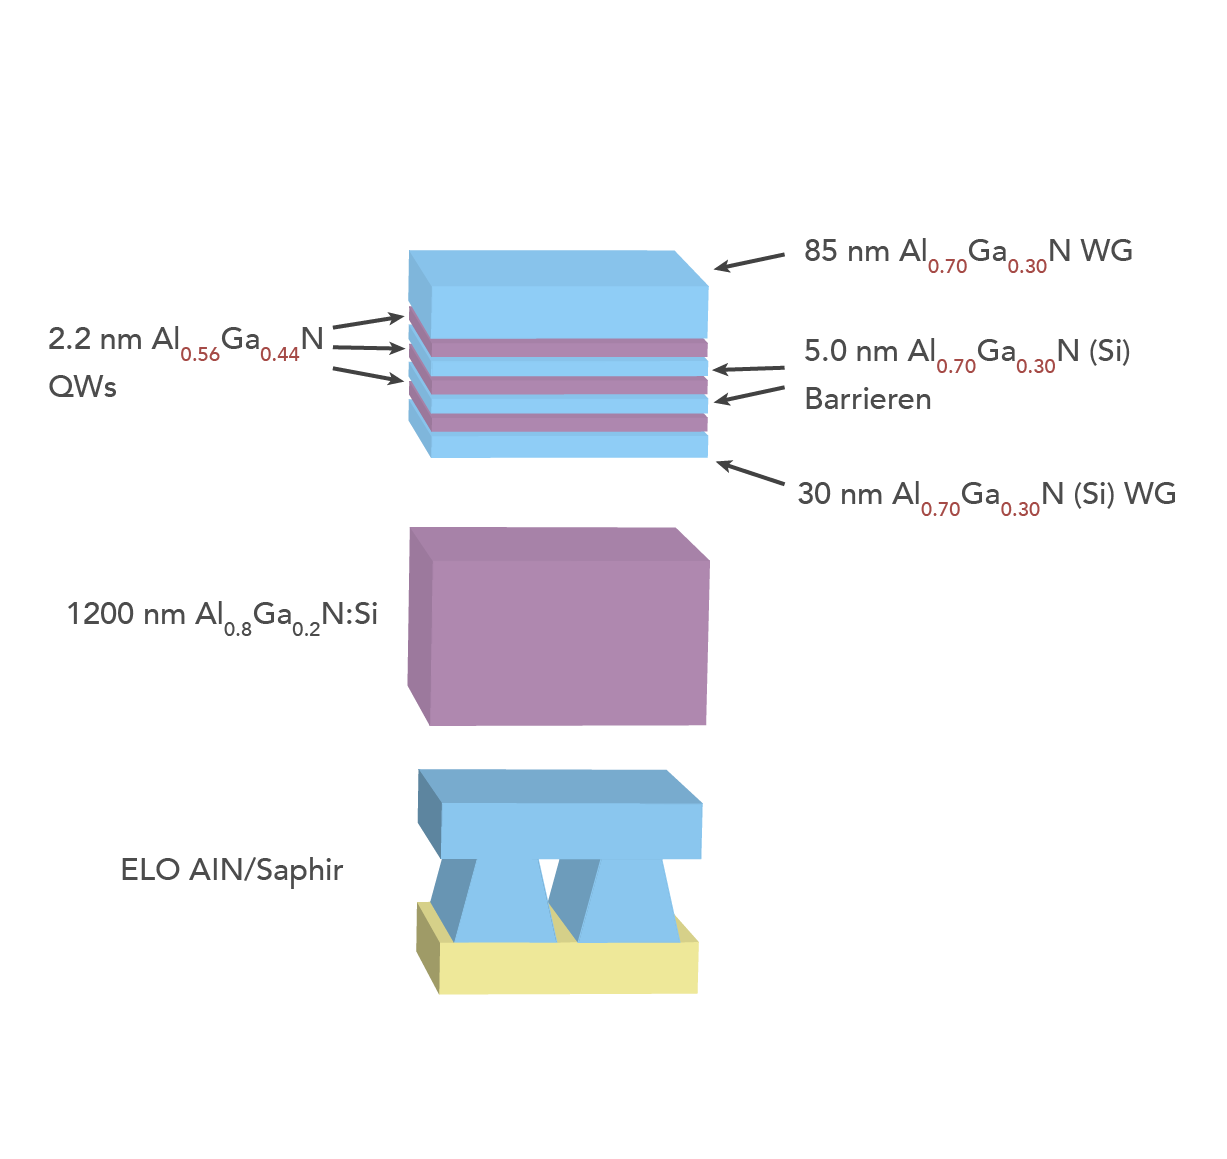
\includegraphics[width=\linewidth]{Bilder/TS4045/ts4045.png}
\caption{Schichtstruktur der untersuchten Proben.}
\label{fig:schichtenelo}
\end{figure}
\noindent 
%
Die drei untersuchten Proben A-ELO, B-ELO und C-ELO setzen sich zusammen aus der oben genannten aktiven Zone. Das Substrat ist ELO AlN/Saphir und darauf aufgewachsen wurde eine $1200 \thinspace nm$ dicke $ Al_{0.8}Ga_{0.2}N$-Bufferschicht (Abb. \ref{fig:schichtenelo}). Die zentrale Wellenlänge der Proben befindet sich bei $(271 \pm 1) \thinspace nm$ wie in Abbildung \ref{fig:spectraselo} zu sehen ist. Durch die nicht resonante Anregung ist der QW-Peak und auch der QB-Peak bei Tieftemperatur bei allen Proben zu sehen, der Anteil des QB-Peaks sinkt aber mit steigender Temperatur durch die steigende kinetische Energie der Elektronen, die bevorzugt in die Leitungsbandminima (den QWs) wandern (thermisches Diffundieren).
%
\begin{figure}[htb]
  \centering
  \begin{minipage}[t]{0.4\textwidth}
    \centering
    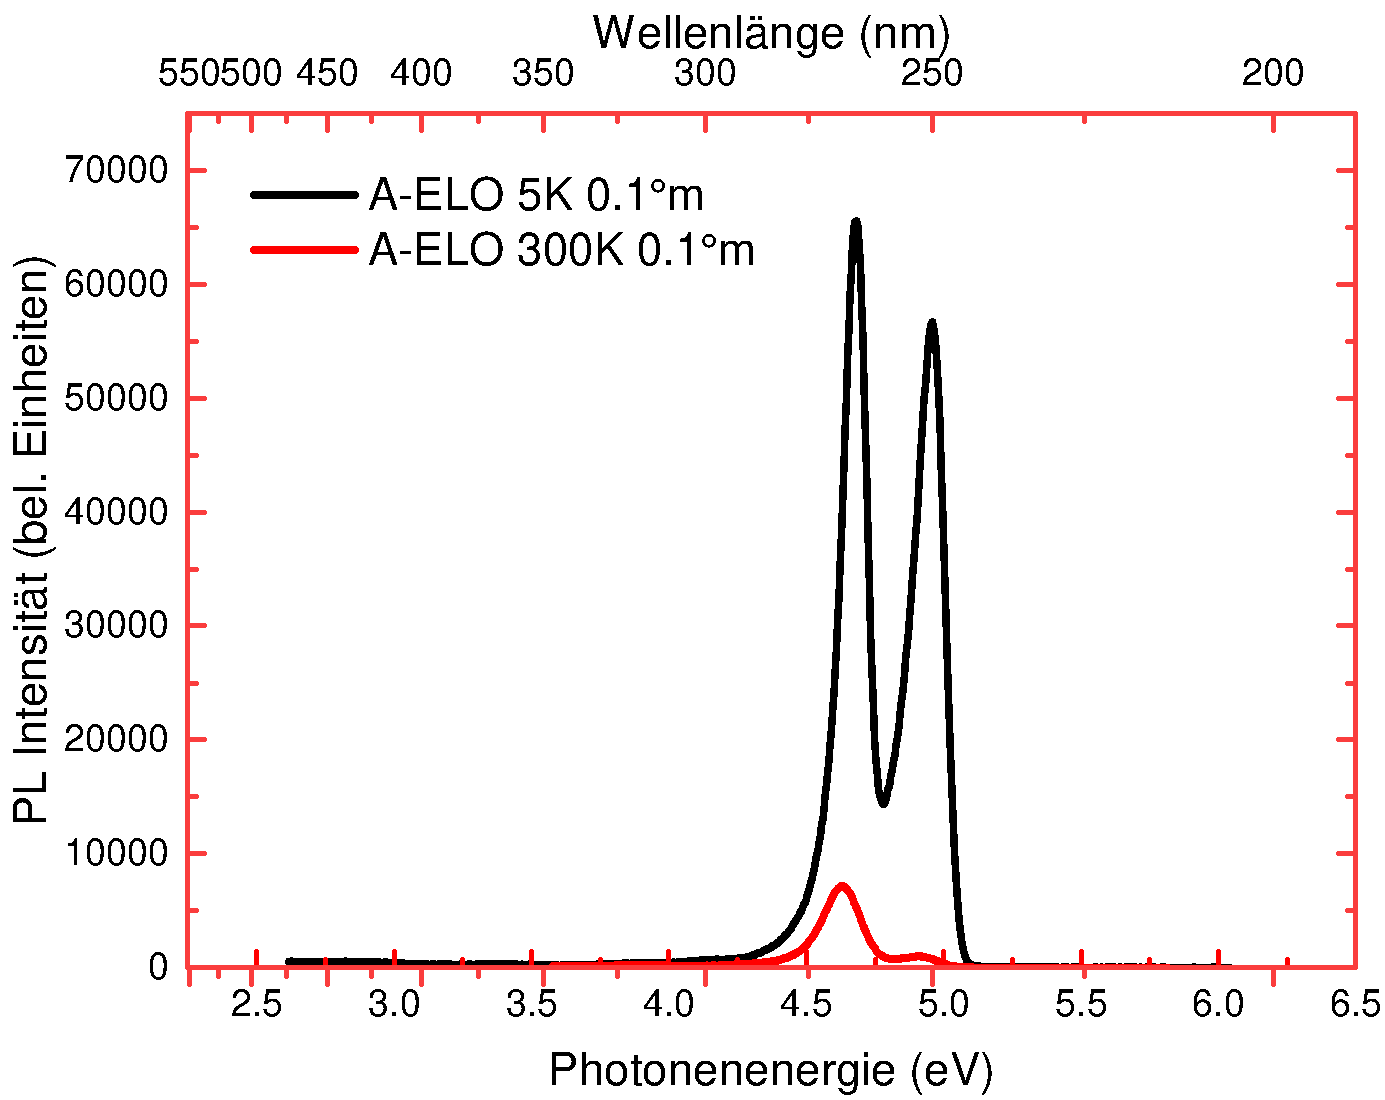
\includegraphics[width=\textwidth]{Bilder/TS4045/aelo.pdf}
  \end{minipage}
	\hfill
  \begin{minipage}[t]{0.4\textwidth}
    \centering
    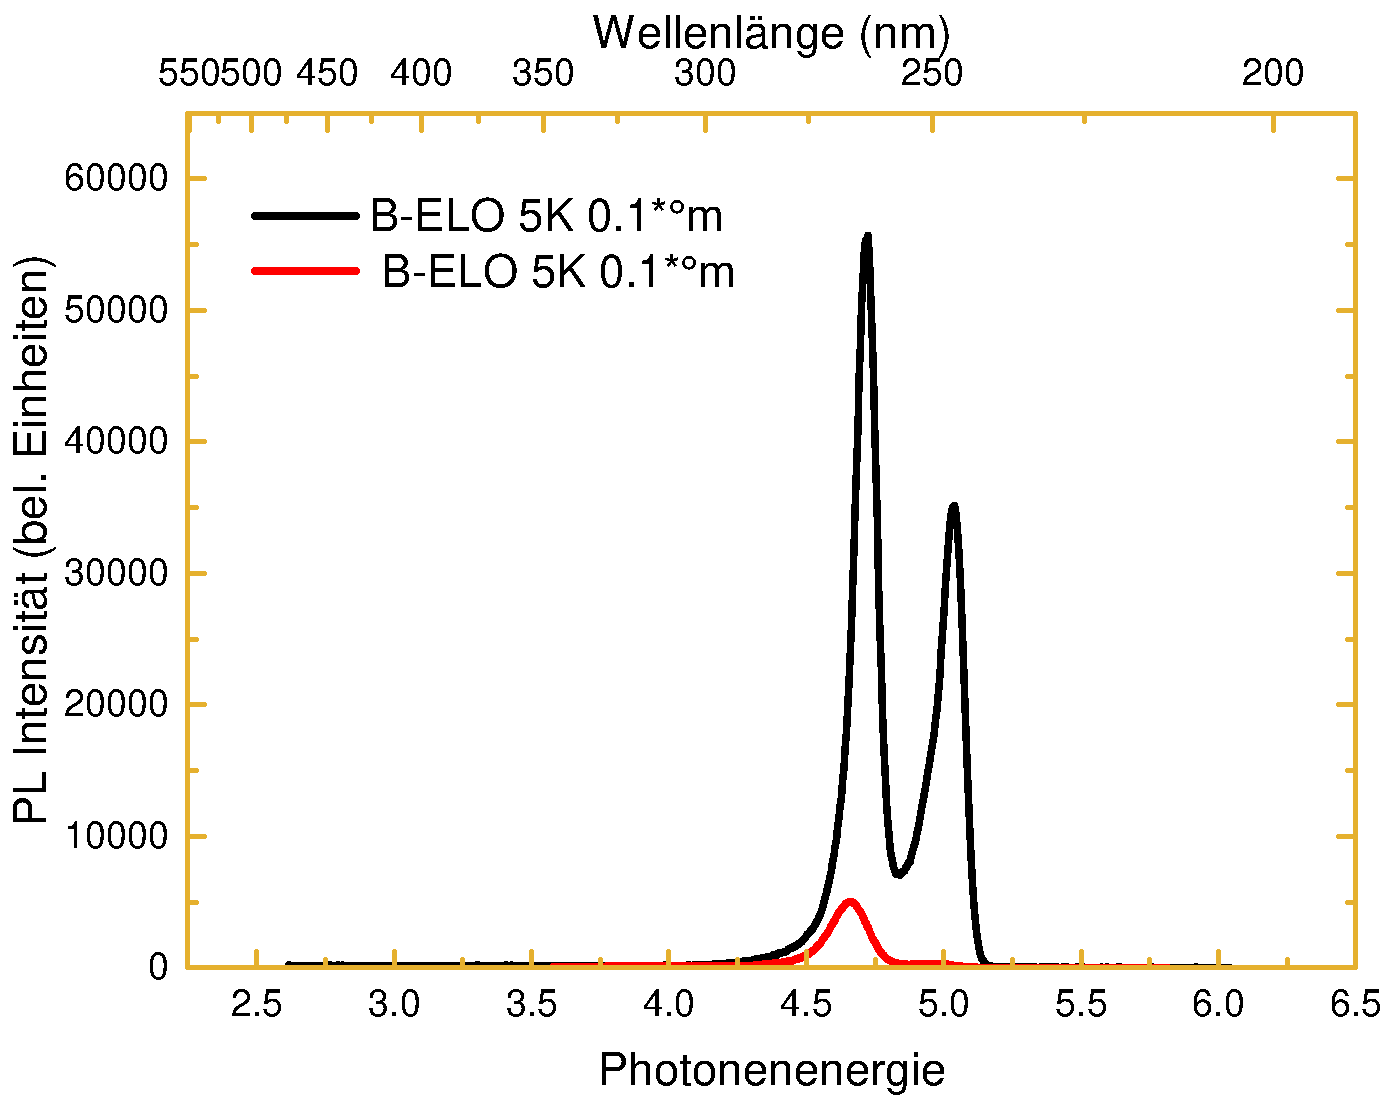
\includegraphics[width=\linewidth]{Bilder/TS4045/belo.pdf}
  \end{minipage}
	\hfill
  \begin{minipage}[t]{0.4\textwidth}
    \centering
    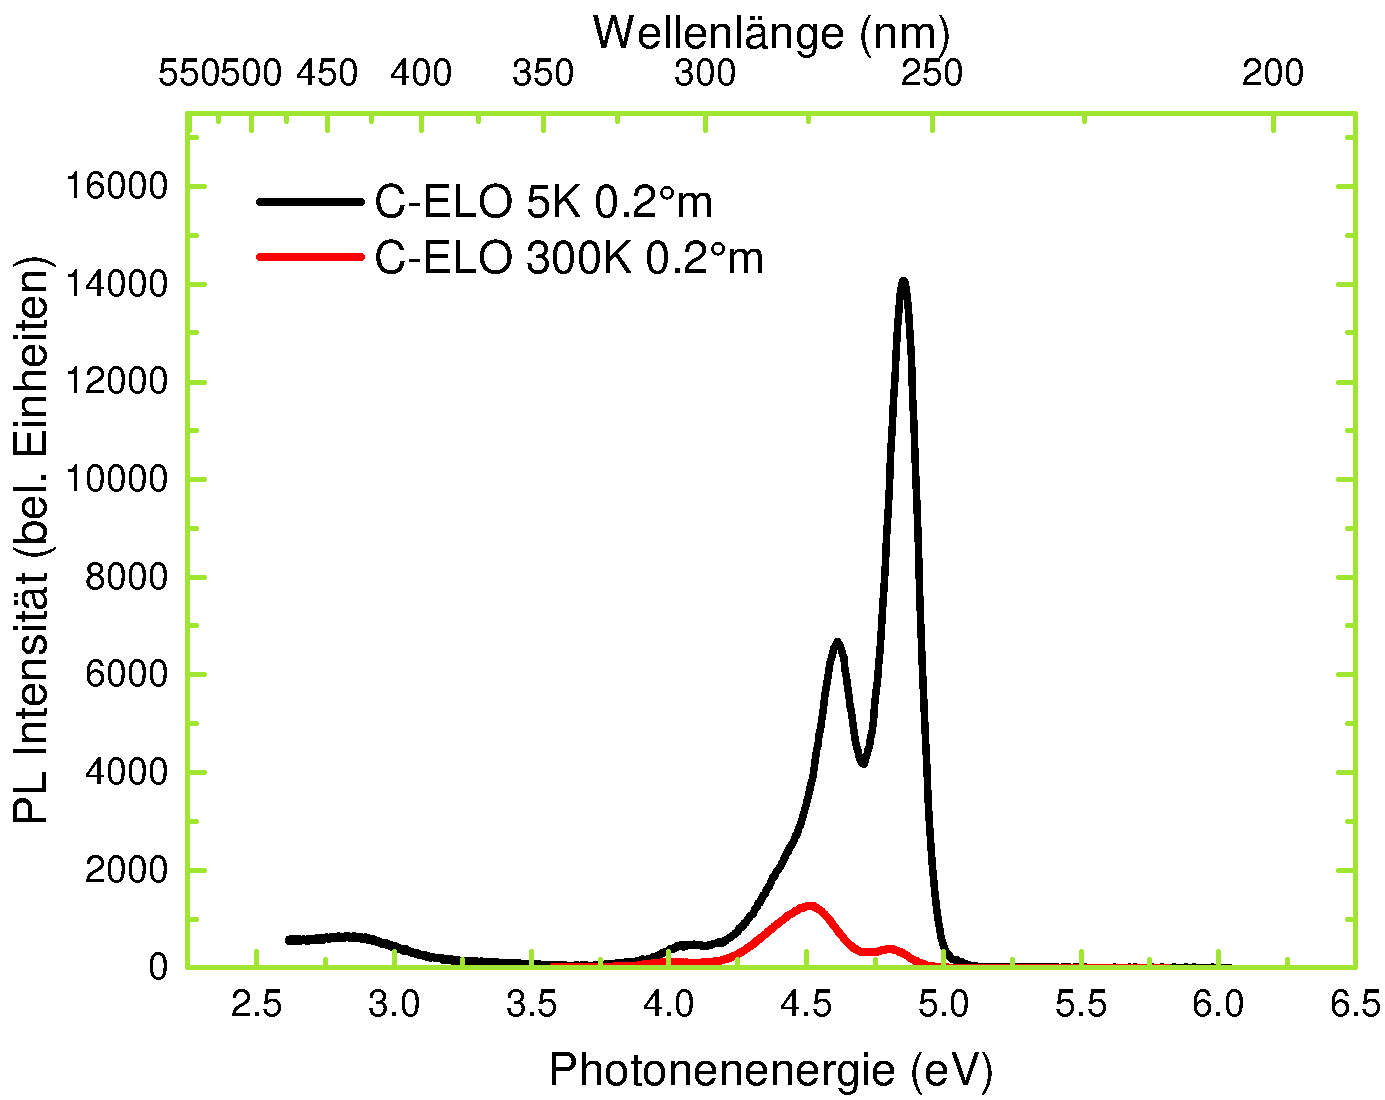
\includegraphics[width=\linewidth]{Bilder/TS4045/celo.pdf}
  \end{minipage}
	\caption{Aufnahme der Spektren der Proben A-ELO mit einem Fehlschnittwinkel von $0.1$ in die Standard m-Richtung, Probe B-ELO mit einem Fehlschnittwinkel von $0.1$ die andere m-Richtung und Probe C-ELO mit einem Fehlschnittwinkel von $0.2$ in die standard m-Richtung. }
	\label{fig:spectraselo}
\end{figure}
\noindent 
%
Die Probe C-ELO zeigt bei TT ein abweichendes Verhalten bezüglich der Verteilung der Intensität auf QB-Peak und QW-Peak. Ein möglicher Grund könnte die Fokussierung sein oder der oberste Waveguide der den gleichen Al-Gehalt hat wie die QBs, absorbiert einen Großteil des Lichtes bevor es in die QWs gelangt. 
Anhand der Intensitäten allein, ist noch kein Rückschluss auf die IQE der Proben zu schliessen., bedingt durch die unterschiedliche Positionierung der Proben und der Fokussierung. Dennoch ist hier bereits auffällig, dass die Probe C-ELO (grün) eine deutlich geringere Intensität bei RT und TT hat.
%
\begin{figure}[htb]
  \centering
  \begin{minipage}[t]{0.49\textwidth}
    \centering
    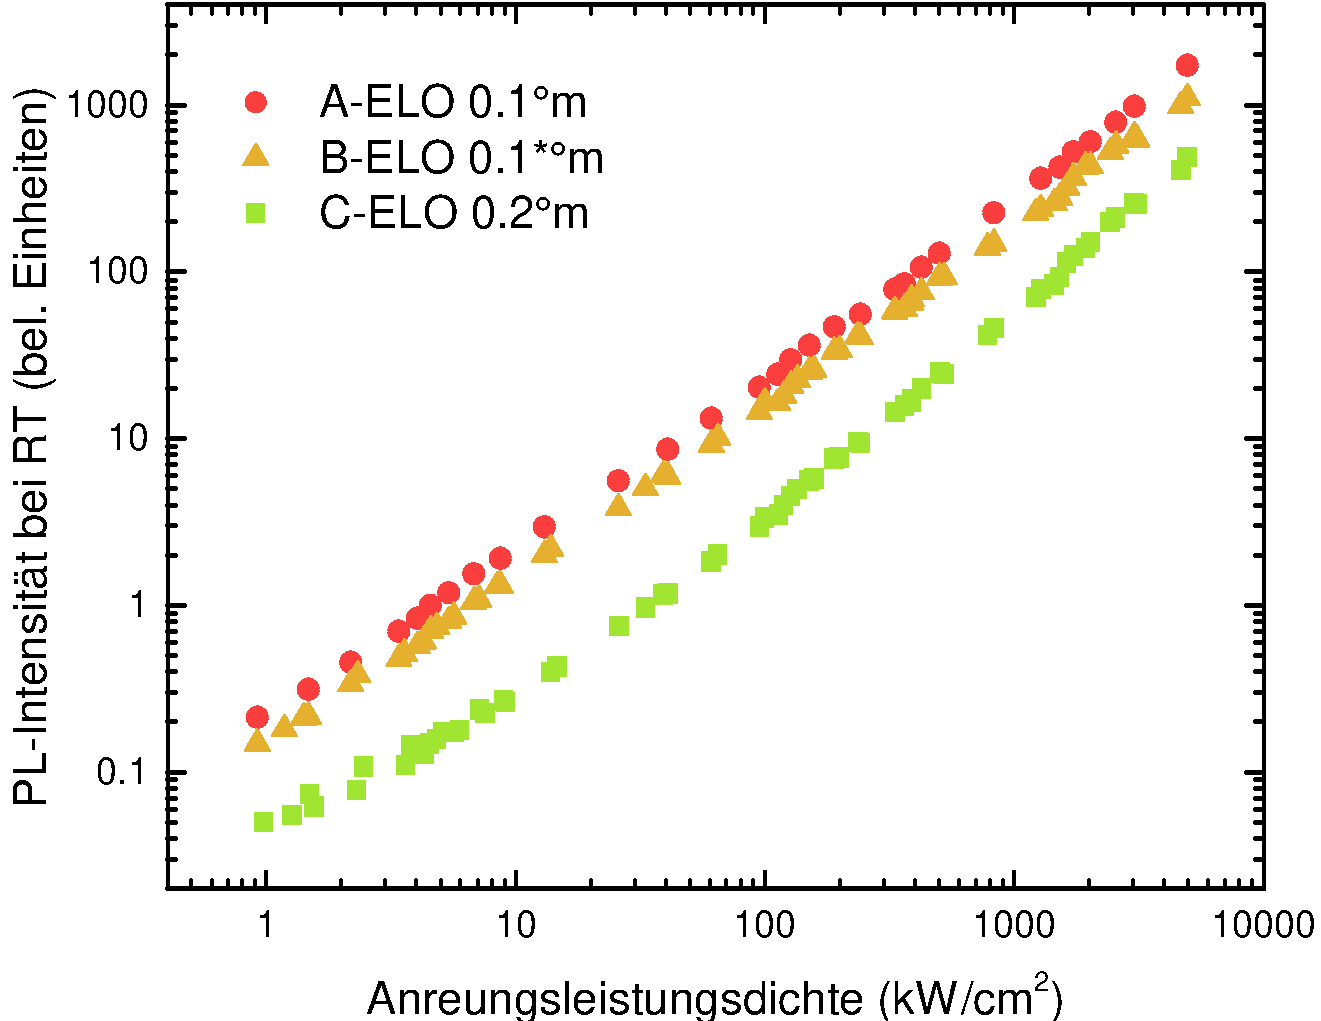
\includegraphics[width=\textwidth]{Bilder/TS4045/intRT.pdf}
		\caption{Die integrierte Intensität in Abhängigkeit der Anregungsleistungsdichte bei Raumtemperatur in doppelt-logarithmischer Darstellung.}
    \label{fig:eloINTrt}
  \end{minipage}
	\hfill
  \begin{minipage}[t]{0.49\textwidth}
    \centering
    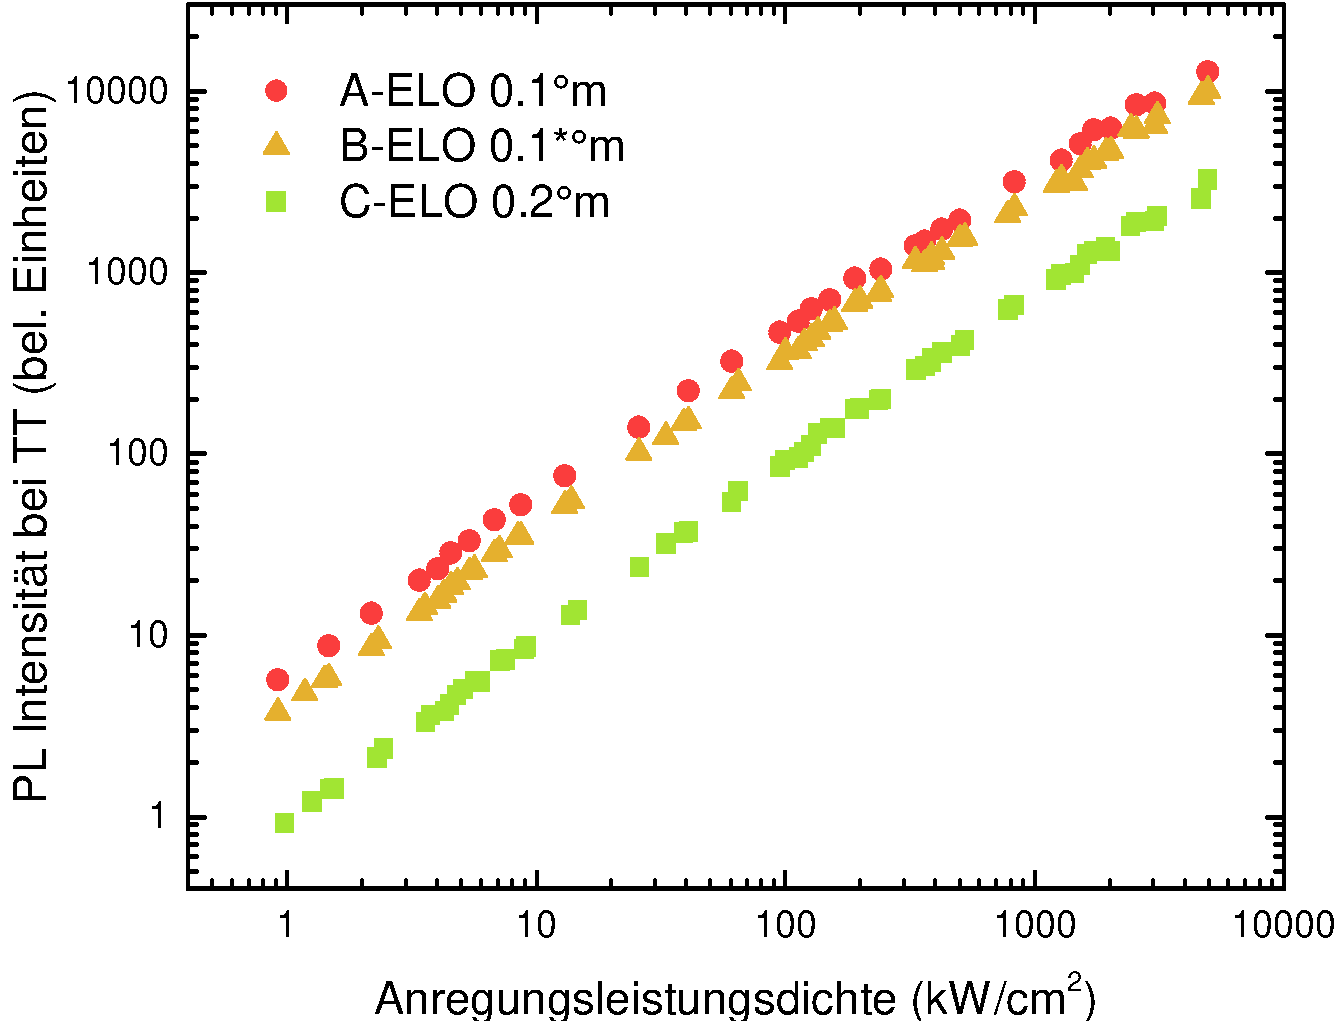
\includegraphics[width=\linewidth]{Bilder/TS4045/intTT.pdf}
		\caption{Die integrierte Intensität in Abhängigkeit der Anregungsleistungsdichte bei Tieftemperatur in doppelt-logarithmischer Darstellung.}
    \label{fig:eloINTtt}
  \end{minipage}
\end{figure}
\noindent 
% 
Dies bestätigt sich in den Abbildungen \ref{fig:eloINTrt} und \ref{fig:eloINTtt}. Die Proben A-ELO und B-ELO zeigen keinen signifikanten Unterschied in den Intensitäten zueinander, der Rückschlüsse auf unterschiedliche IQEs erlauben würde. Bei der Probe C-ELO könnte vermutet werden, anhand der drastischen Unterschiede in den Intensitäten der Spektren, dass sie die geringste IQE hat, da sie mit deutlichem Abstand am schwächsten leuchtet, obwohl bei allen Proben die gleiche Fläche beleuchtet wird. 
%
\begin{figure}[H]
  \centering
  \begin{minipage}[t]{0.49\textwidth}
    \centering
    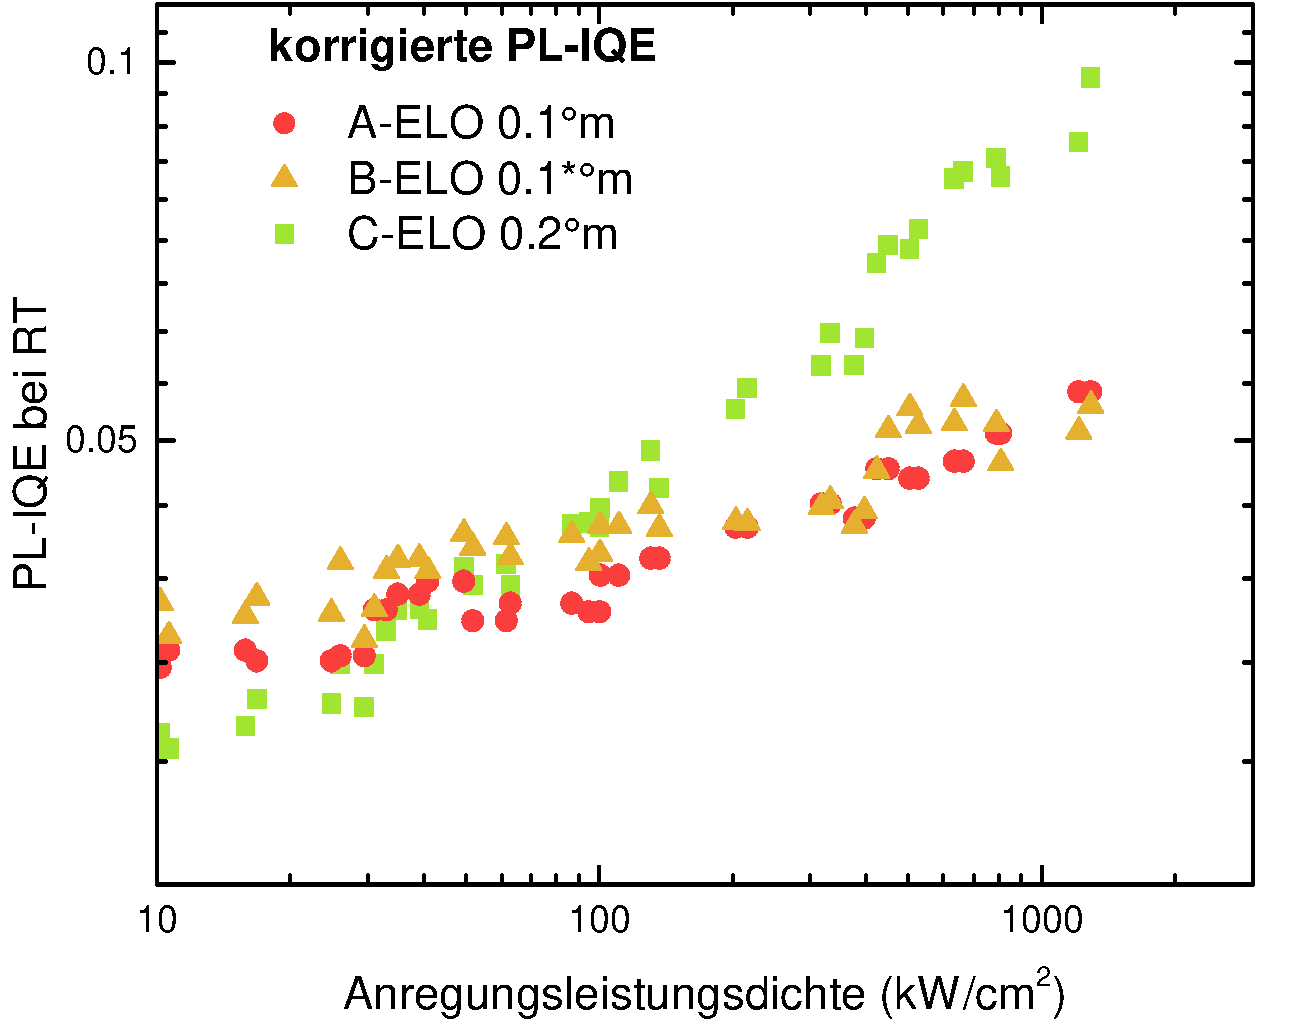
\includegraphics[width=\textwidth]{Bilder/TS4045/corrIQERT.pdf}
		\caption{Die IQEs für die Proben A-ELO, B-ELO und C-ELO bei Raumtemperatur.}
    \label{fig:eloiqeRT}
  \end{minipage}
	\hfill
  \begin{minipage}[t]{0.49\textwidth}
    \centering
    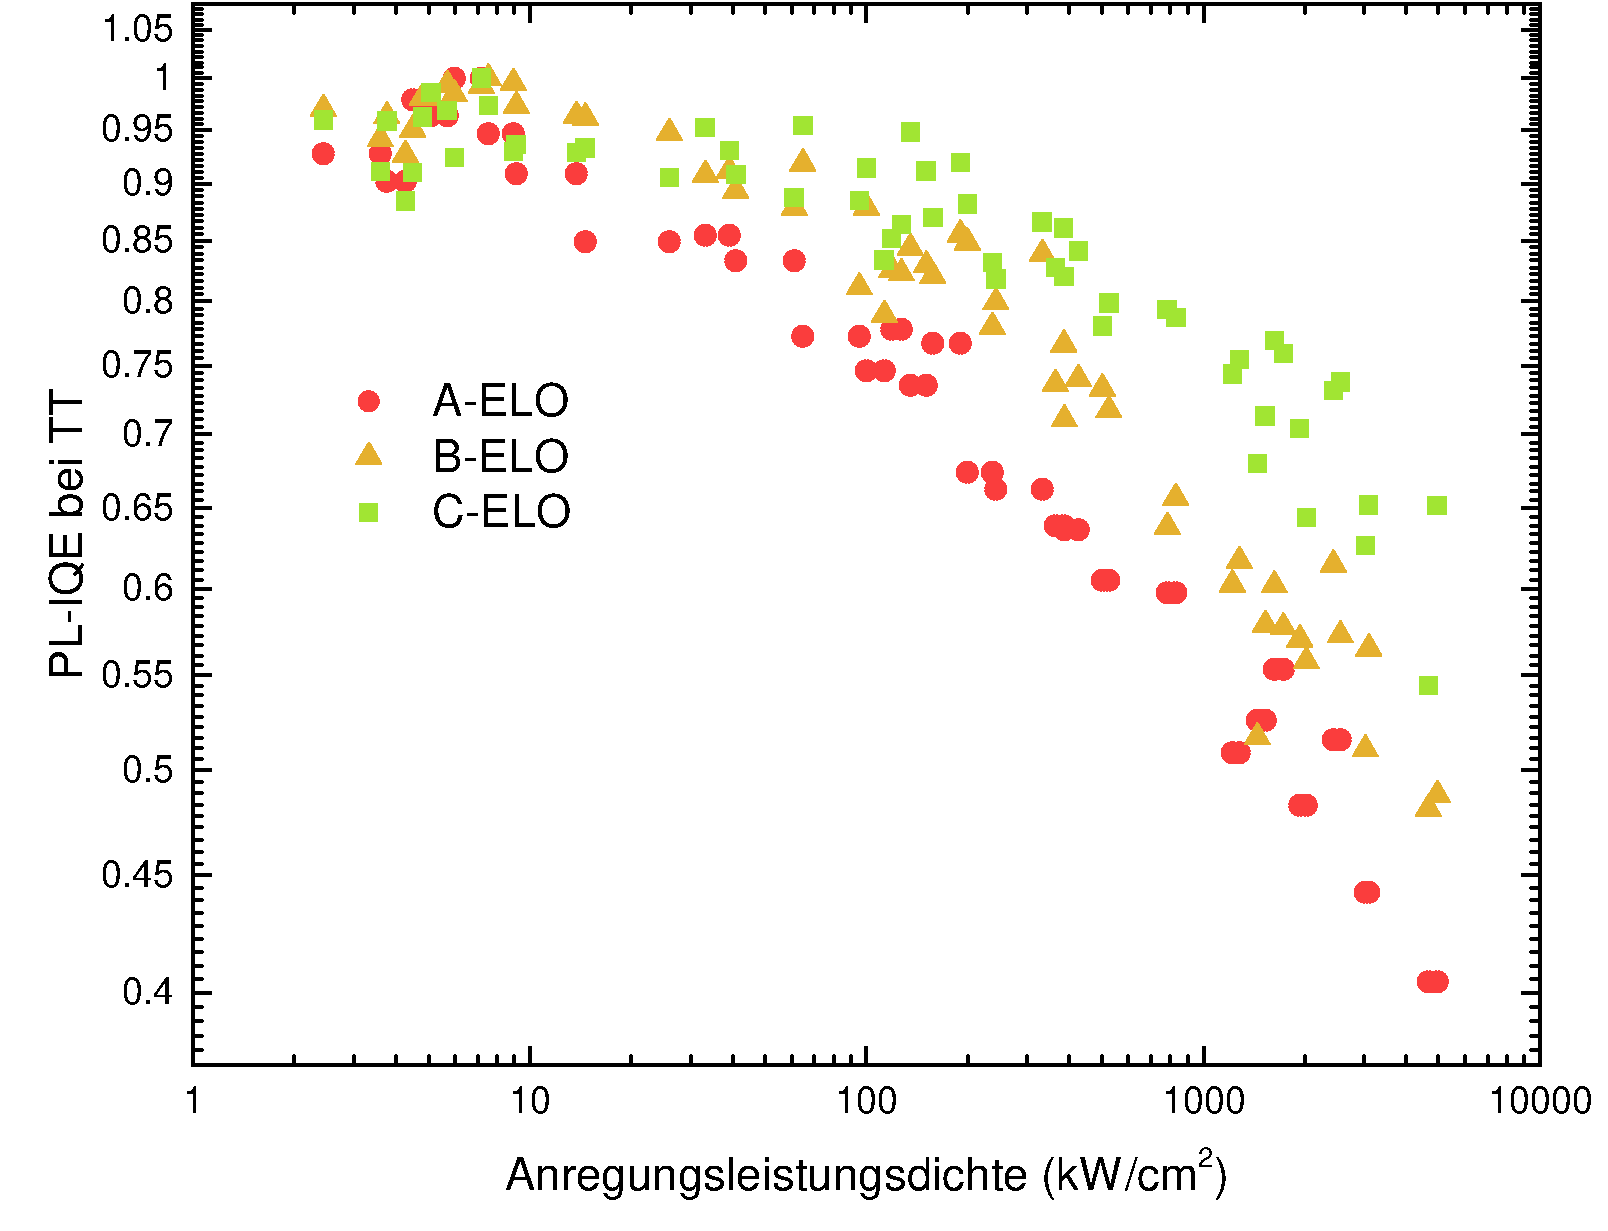
\includegraphics[width=\linewidth]{Bilder/TS4045/IQETT.pdf}
		\caption{Die IQEs für die Proben A-ELO, B-ELO und C-ELO bei Tieftemperatur.}
    \label{fig:elocorriqeRT}
  \end{minipage}
\end{figure}
\noindent 
%
Die Ergebnisse für die IQE bei RT sind in Abbildung \ref{fig:eloiqeRT} zu sehen. Die IQE Probe C-ELO ist mit einem Wert von $IQE_{C-ELO} = 0,028$ im Bereich von geringen Anregungsleistungsdichten von $ 10 \frac{kW}{cm^2} $ bis $ 100 \frac{kW}{cm^2} $ niedriger als für die Proben A-ELO und B-ELO, die sich, wie aus den Intensitäten und ihren Verhältnissen bei TT und RT bereits zu vermuten ist, ähnlich verhalten. 
Die IQE für die Probe C-ELO weist indes eine deutlich stärkere Steigung auf, sodass die IQE mit zunehmender Anregungsleistungsdichte die der Proben A-ELO und B-ELO immer deutlicher übersteigt. Sodass bei der höchsten Anregungsleistungsdichte $ 1300 \frac{kW}{cm^2} $ die IQE der Probe C-ELO mit einer IQE von $IQE_{C-ELO} = 0,098$ (9,8 \%) die der Proben A-ELO mit $IQE_{A-ELO} = 0,055$ (5,5 \%) und B-ELO mit $IQE_{B-ELO} = 0,054$ (5,4 \%) um fast das doppelte übersteigt. Werden zusätzlich die IQEs bei $5K$ berachtet, ist ersichtlich, dass die IQEs Proben A-ELO und B-ELO erheblich schneller absinken als die der Probe C-ELO. Dieser erreicht mit sinkender Anregungsleistungsdichte das Plataeu , dass bei geringen Anregungsleistungen aufgrund der $n^3$ Abhängigkeit der Auger-Rekombination zu erwarten ist. A-ELO und C-ELO dagegen scheinen dieses Plataeu nicht zu erreichen. Daraus resultierend, liegt die Schlussfolgerung nahe, dass die hier verwendeten Anregungsleistungsdichten für die Proben A-ELO und B-ELO nicht gering genug und somit die IQEs unterbewertet sind, zudem ist das unterschiedliche Verhalten der IQEs bei $5K$ möglicherweise dadurch zu erklären, dass auf die Probe C-ELO nicht die gleiche Anzahl an Ladungsträgern die aktive Zone erreichen. Was im Umkehrschluss erklärt, wieso das Plataeu bei der Probe C-ELO früher erreicht wird, da somit die tatsächlich auf der Probe ankommende Anregungsleistungsdichte geringer ausfällt.  
%
\begin{figure}[H]
\begin{tabular}{ccc}
  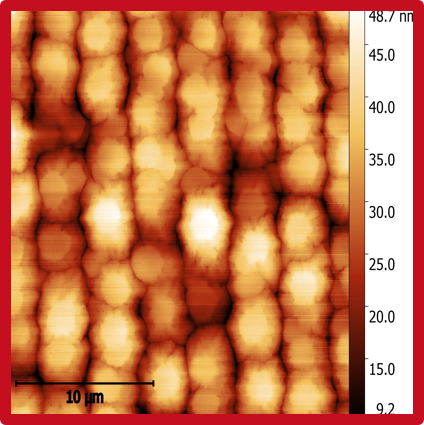
\includegraphics[width=0.30\textwidth]{Bilder/TS4045/aELOafm.png} & 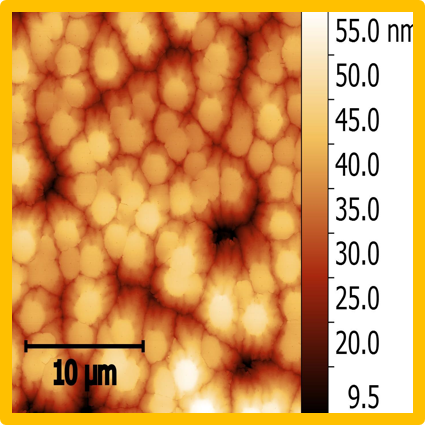
\includegraphics[width=0.30\textwidth]{Bilder/TS4045/bELOafm.png}  & 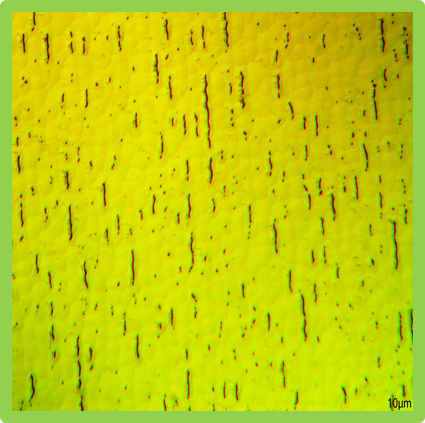
\includegraphics[width=0.30\textwidth]{Bilder/TS4045/cELOlimi.png} \\
(a) & (b) & (c) \\[6pt]
 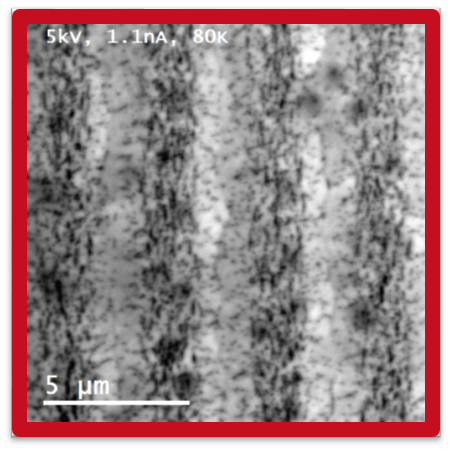
\includegraphics[width=0.30\textwidth]{Bilder/TS4045/aELOcl2.png} &   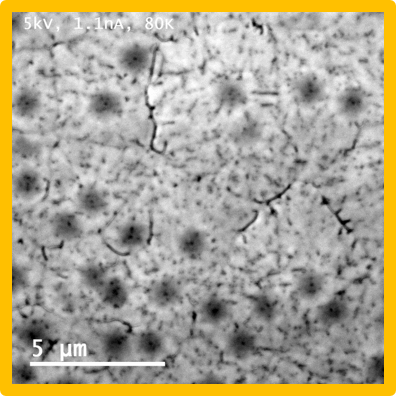
\includegraphics[width=0.30\textwidth]{Bilder/TS4045/bELOcl2.png} & 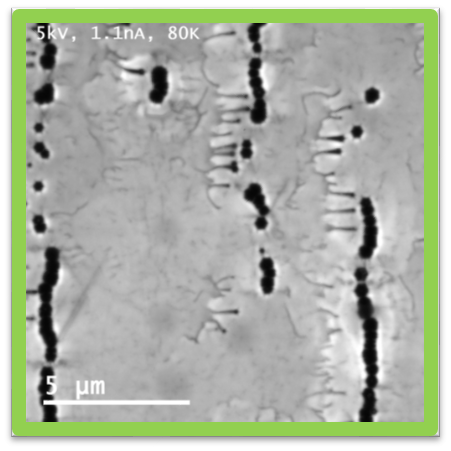
\includegraphics[width=0.30\textwidth]{Bilder/TS4045/cELOcl2.png}  \\
(d)  & (e) & (f)   \\[6pt]
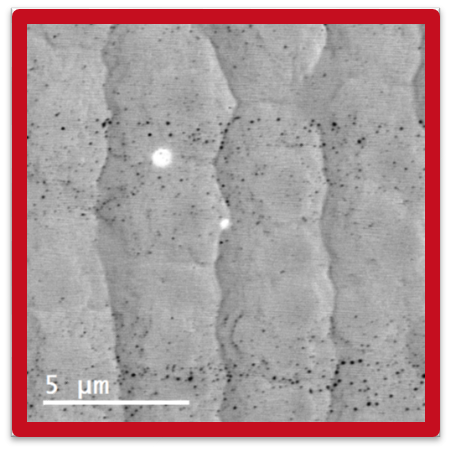
\includegraphics[width=0.30\textwidth]{Bilder/TS4045/aELOcl1.png} & 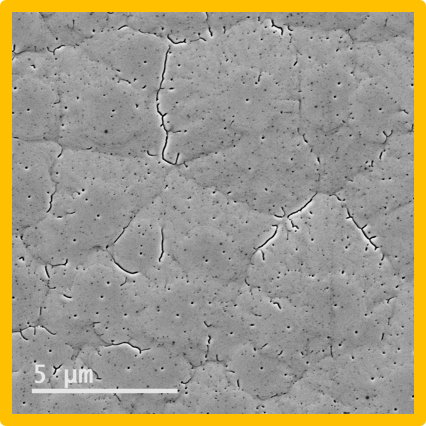
\includegraphics[width=0.30\textwidth]{Bilder/TS4045/bELOcl1.png}  & 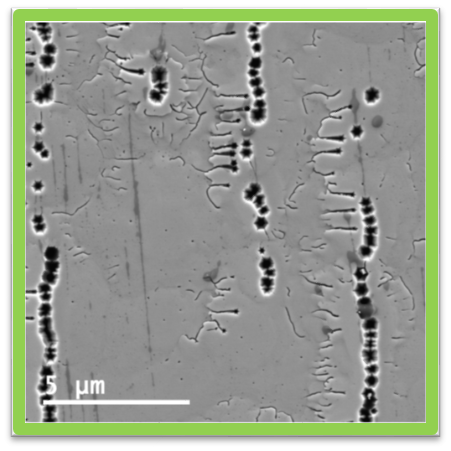
\includegraphics[width=0.30\textwidth]{Bilder/TS4045/cELOcl1.png} \\
(g)  & (h) & (i)   \\[6pt]
\end{tabular}
\caption{AFM-Bilder (a, b) und eine Limi-Aufnahme (c) von Christian Kuhn aufgenommen. SEM (c, d, e) und panchromatische CL-Aufnahmen(f, g, h) an den selben Stellen gemessen von Ute Zeimer (FBH)}
\label{fig:morph1}
\end{figure}
\noindent 
Um die Gründe für diese Unterschiede in den IQEs und den Einfluss des Fehlschnittes auf die Oberflächenmorphologie weiter zu untersuchen, werden AFM-Aufnahmen und panchromatische CL-Aufnahmen und dazu von derselben Stelle Rasterelektronenmikroskopie-Aufnahmen betrachtet und auf ihre Besonderheiten analysiert. Die CL-Bilder wurden bei einer Beschleunigungsspannung von 5 kV,
einer Stromstärke von 1,1 nA und einer 5000-fachen Vergrößerung von Ute Zeimer aufgenommen.
Auf den AFM-Aufnahmen der Probe A-ELO in Abbildung \ref{fig:morph1} (a) sind entlang der ELO-Streifen Spiralen zu sehen und die SEM-Aufnahme (c) zeigen Wachstumssinseln und eine glatte Oberfläche. Die panchromatischen CL-Aufnahmen zeigen eine Verteilung dunkler Punkte (engl.: dark spot) hauptsächlich an den Kämmen der ELO-Streifen zwischen den geätzten Gräben. Diese korrelieren direkt mit Schraubenversetzungen die bis an die Oberfläche reichen. Auf der AFM-Aufnahme der Probe B-ELO (b) sehen wir statt den Spiralen auf den ELO-Streifen dagegen zufällig verteilte Spiralen. Der Grund dafür liegt hauptsächlich an dem Einfluss der unterschiedlichen Richtungen der ELO-Streifen zu der Fehlschnittrichtung. Die SEM-Aufnahme (g) zeigt viele Hohlräume und Risse an der Oberfläche. Auf dem panchromatischen CL-Bild (d) sind die dunklen Punkte verstreut auf der Oberfläche zu sehen. 
Die Oberfläche der Probe C-ELO dagegen weist, wie auf Abbildung (c) zu sehen ist, viele Gruben (engl.: pits) entlang der ELO Streifen auf. Das ELO ist zwar koalesziert, aber beim Wachstum der MQWs ist wahrscheinlich etwas schief gelaufen. Zudem ist wieder erwarten kein Stufenbündelwachstum zu sehen. Mit diesem Wissen lässt sich sagen, dass die Proben A-ELO und B-ELO mit dem gleichen Fehlschnitt in verschiedene Richtungen sich in ihren Emissions-Eigenschaften ähnlich verhalten und die IQEs mit 5,4 \% und 5,5 \% sich gleichen. Allerdings äußert sich an der Morphologie eindeutig der Einfluss der Fehlschnitt-Richtung zur Richtung der ELO Streifen.
Die Ergebnisse der Probe C-ELO dagegen lassen sich schwer interpretieren. Sie besitzt eine fast doppelt so hohe IQE wie die anderen beiden Proben, bei einer geringeren Intensität. Auf der Probe selbst scheinen weniger Elektron-Loch-Paare generiert zu werden, was sich durch eben eine geringere Intensität äußert, aber untermauert wird durch die IQE bei $5K$ und dem bei weitem früher einsetzenden Plateau. Die Gründe dafür können schwer bestimmt werden. Beim Wachstum des MQW ist eindeutig etwas schief gelaufen und äußert sich in der Morphologie. Inwieweit die Morphologie einen Einfluss auf die Kollektionseffizienz (Licht- ein- und auskopplung) der 
Proben hat, ist schwierig und zu diesem Zeitpunkt nicht benennbar. So bleibt die IQE der Probe C-ELO ohne weitere Investigation schwer bis gar nicht zu verwerten. Um den tatsächlichen Einfluss eines Fehlschnittwinkels von 0.2$^\circ$ auf die Defektdichte und damit eine IQE zu bestimmen, wäre es notwendig, eine neue Serie zu wachsen bei der das MQW-Wachstum nicht schief lief und zusätzlich Messungen in denen die maximale IQE bestimmt wird. Letzteres ist mit dem derzeitigen PL-Aufbau nicht möglich.


\section{UVC-Laser Strukturen auf ELO mit Übergitter}
\begin{figure}[h]
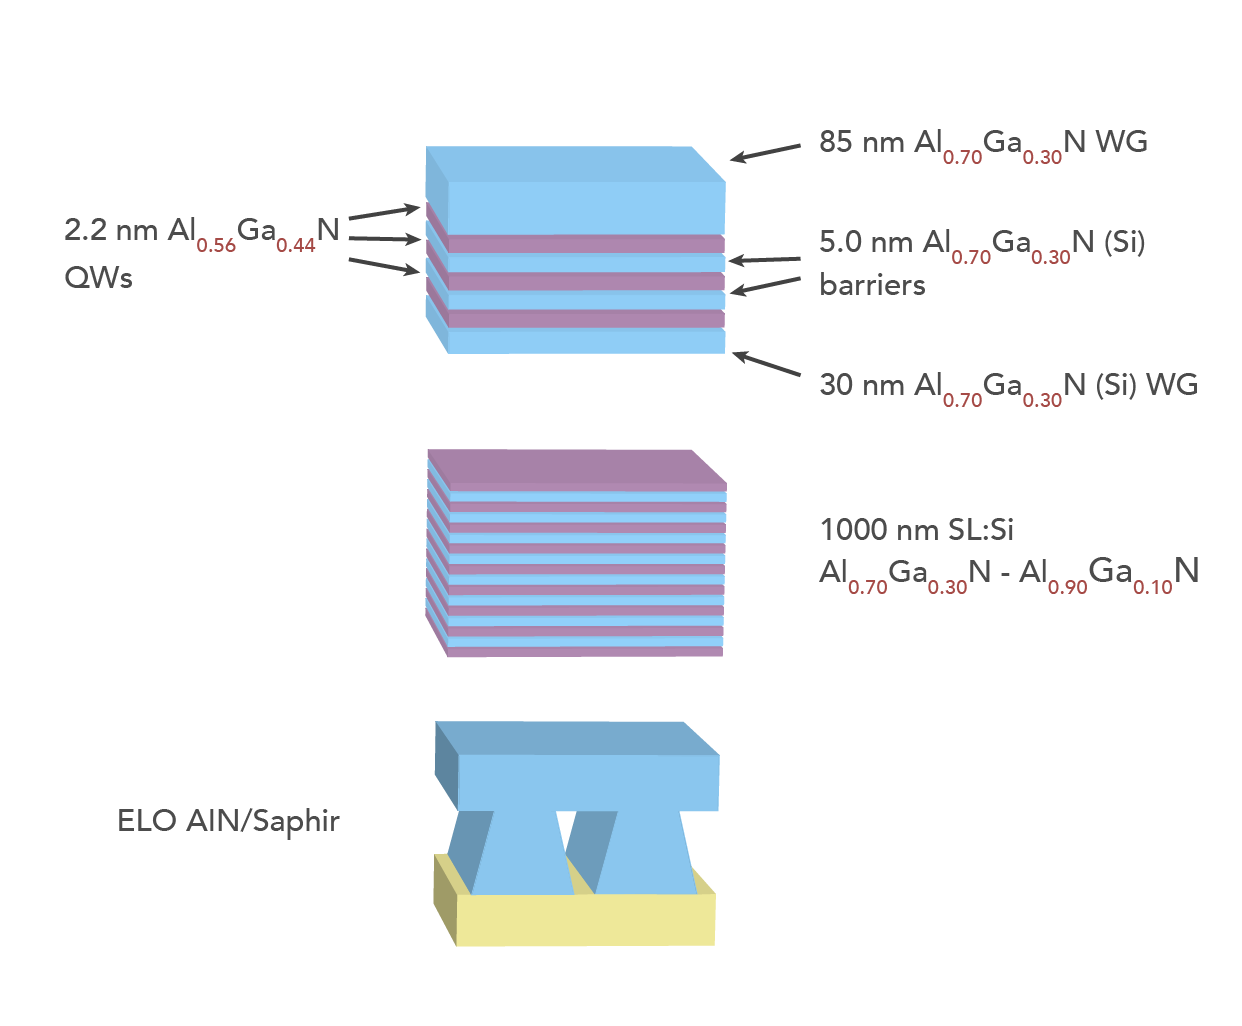
\includegraphics[width=\linewidth]{Bilder/TS4048/ts4048.png}
\caption{Schichtstruktur der untersuchten Proben.}
\label{fig:schichtenelo}
\end{figure}
\noindent 
Die drei untersuchten Proben A-SL-ELO, B-SL-ELO und C-SL-ELO setzen sich zusammen aus der gleichen aktiven Zone. Das Substrat ist ELO AlN/Saphir und darauf aufgewachsen wurde ein $1000 \thinspace nm$ dickes Übergitter aus dünnen alternierenden Schichten aus $ Al_{0.7}Ga_{0.3}N$ und $ Al_{0.9}Ga_{0.1}N$, da so Wachstum von AlGaN-Schichten mit einer verbesserten lateralen Uniformität in der Zusammensetzung und des Spannungszustands ermöglicht wird und so zu einer signifikanten Reduzierung der Oberflächenrauheit führt \cite{doi:10.1002/pssa.201800005} \cite{tino}. Dies ist bei Laserdioden von besonderer Wichtigkeit um optische Streuung, die zu Verlusten im Resonator führt, möglichst zu vermeiden. So ist durch eine glattere Oberfläche eine geringere Laserschwelldichte zu erreichen \cite{doi:10.1002/pssa.201870032}.
%
\begin{figure}[htb]
  \centering
  \begin{minipage}[t]{0.4\textwidth}
    \centering
    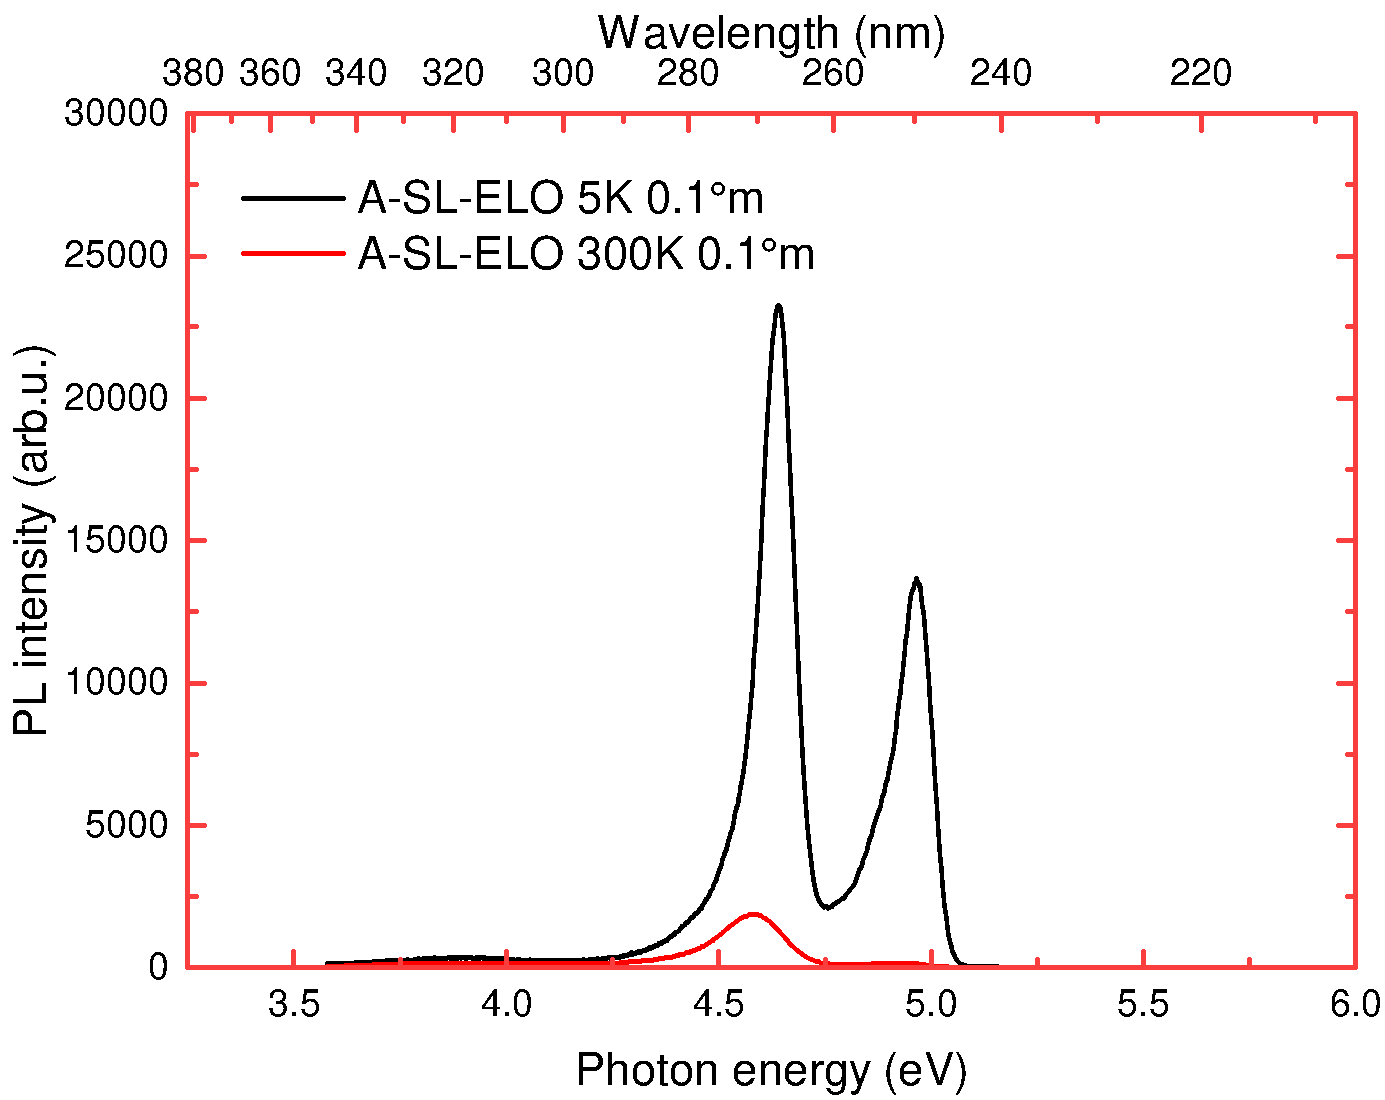
\includegraphics[width=\textwidth]{Bilder/TS4048/aslelo.pdf}
  \end{minipage}
	\hfill
  \begin{minipage}[t]{0.4\textwidth}
    \centering
    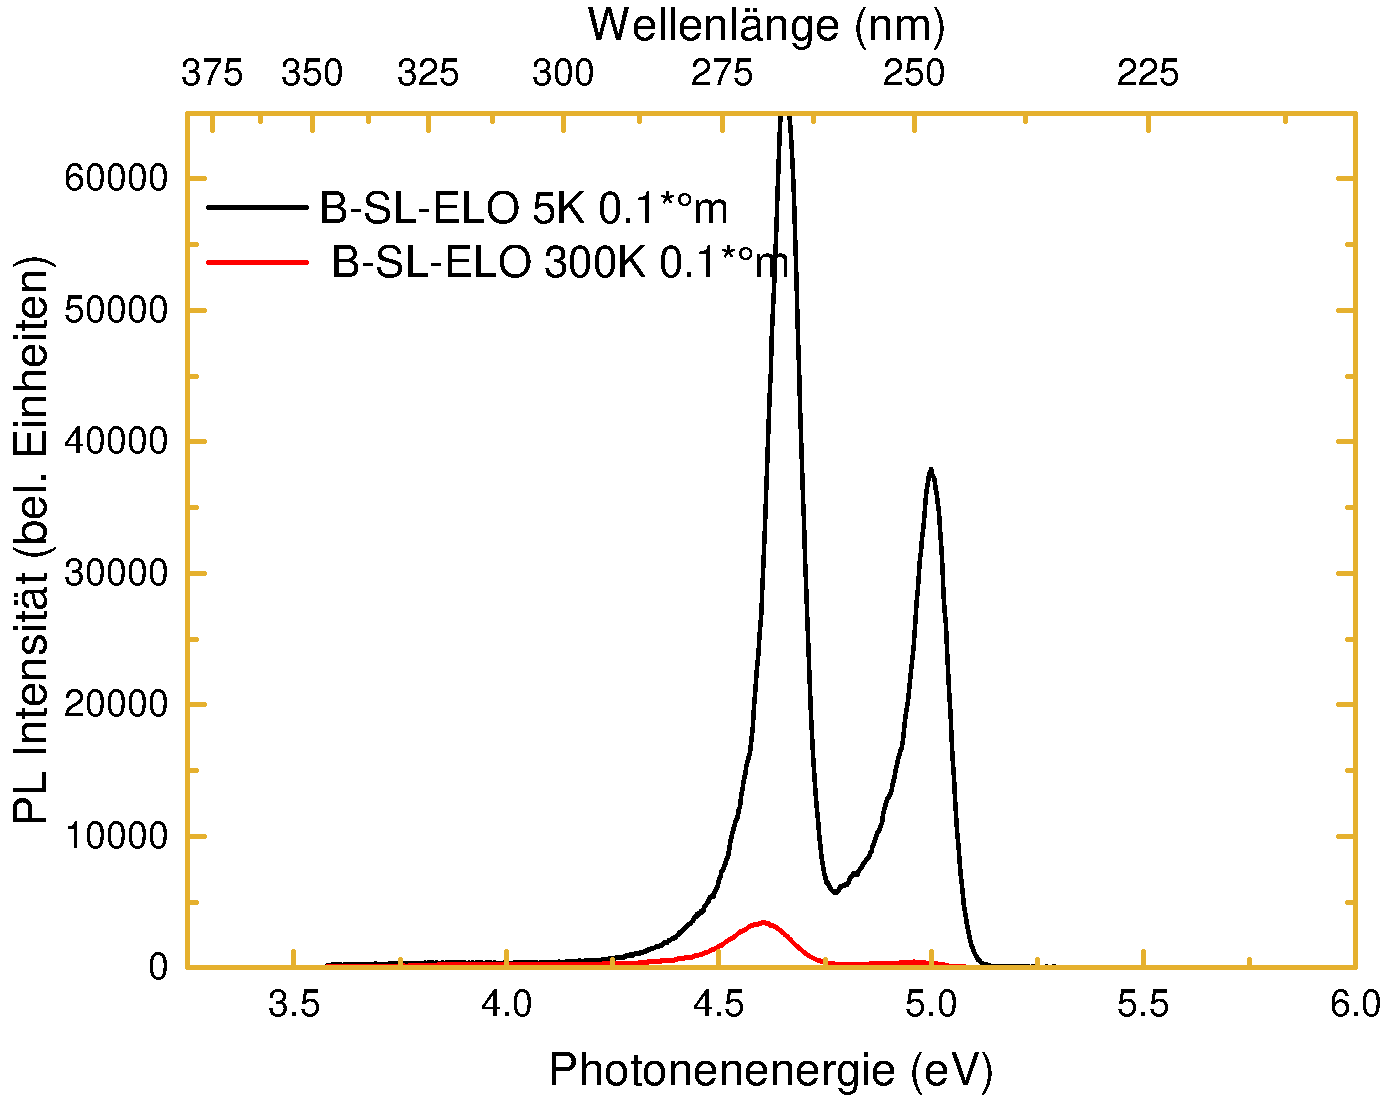
\includegraphics[width=\linewidth]{Bilder/TS4048/bslelo.pdf}
  \end{minipage}
	\hfill
  \begin{minipage}[t]{0.4\textwidth}
    \centering
    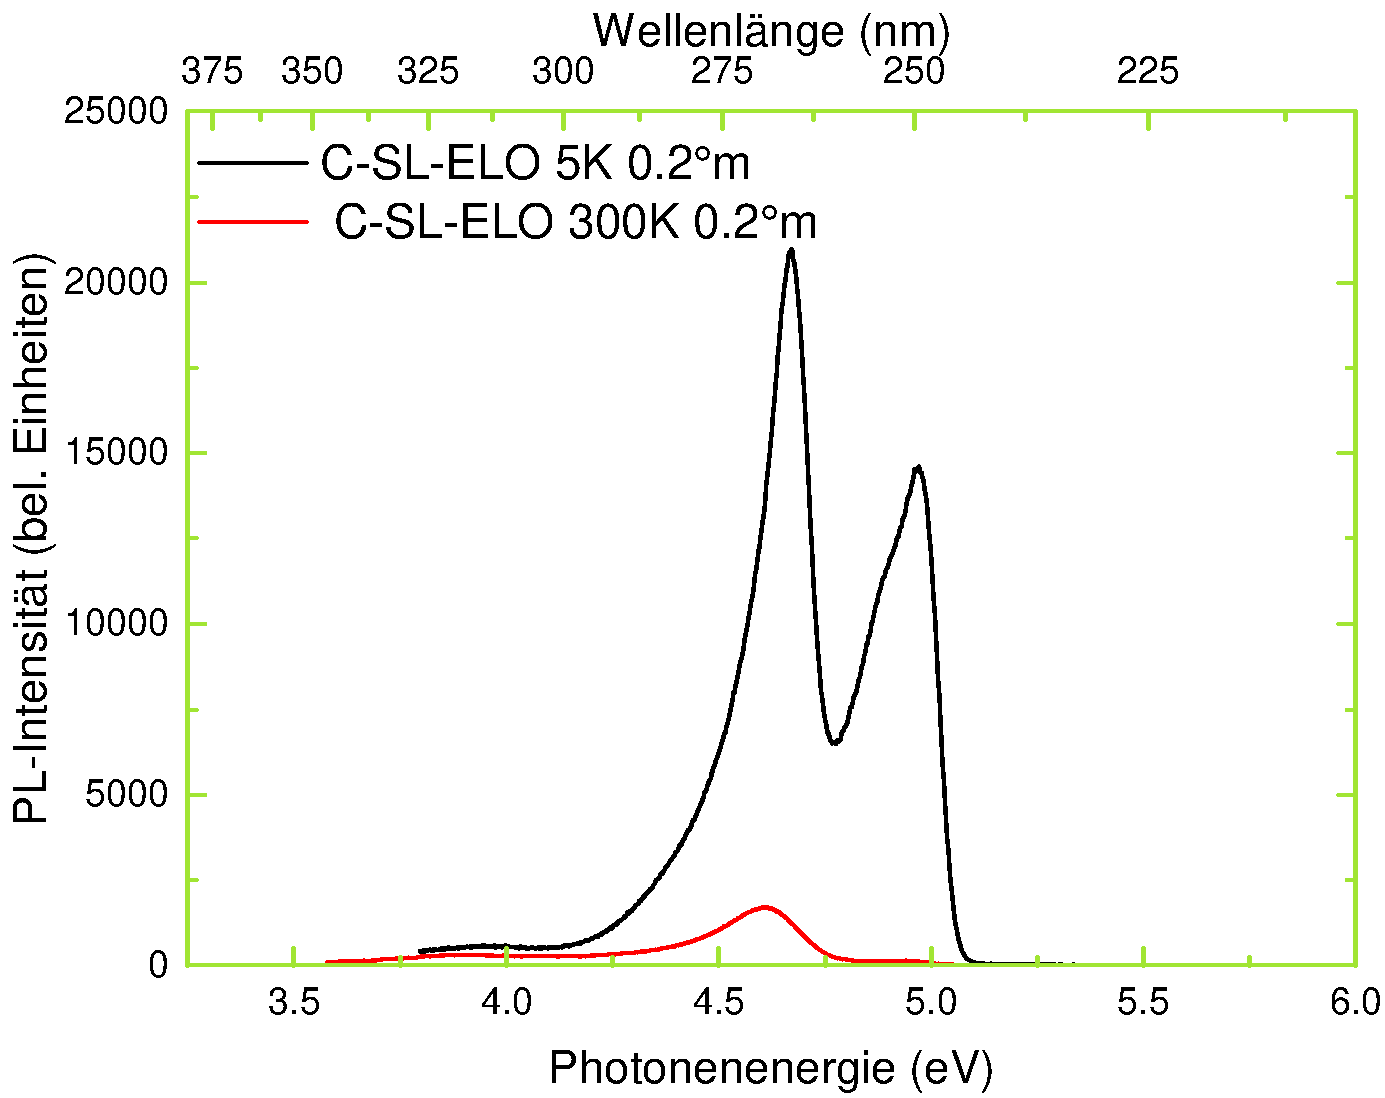
\includegraphics[width=\linewidth]{Bilder/TS4048/cslelo.pdf}
  \end{minipage}
	\caption{Aufnahme der Spektren der Proben A-SL-ELO mit einem Fehlschnittwinkel von $0.1$ in die Standard m-Richtung, Probe B-SL-ELO mit einem Fehlschnittwinkel von $0.1$ die andere m-Richtung und Probe C-SL-ELO mit einem Fehlschnittwinkel von $0.2$ in die standard m-Richtung. }
	\label{fig:spectrassl}
\end{figure}
\noindent 
%
Die Spektren bei $5K$ und $300K$ zeigen keine signifikanten Unterschiede in der Intensität wie in Abbildung \ref{fig:spectrassl} zu sehen ist. Der QB-Peak der Probe C-SL-ELO ist energetisch näher am QW-Peak als bei den anderen Proben und weist eine andere Form auf, nimmt aber keinen Einfluss auf die Ergebnisse der IQE. 
%
\begin{figure}[H]
  \centering
  \begin{minipage}[t]{0.49\textwidth}
    \centering
    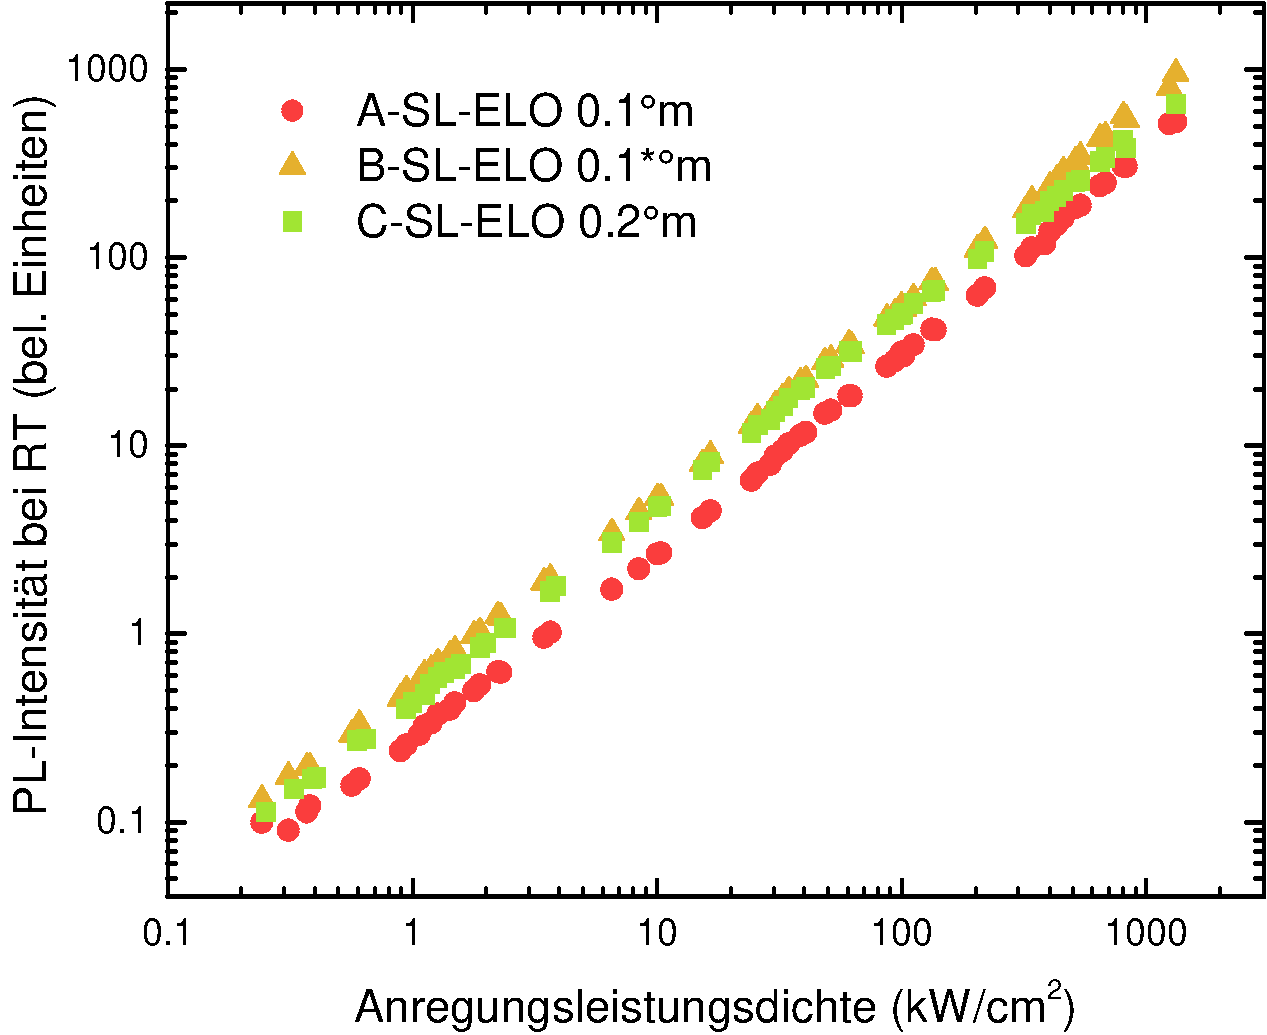
\includegraphics[width=\textwidth]{Bilder/TS4048/intRT.pdf}
		\caption{Die integrierte Intensität in Abhängigkeit der Anregungsleistungsdichte bei Raumtemperatur in doppelt-logarithmischer Darstellung.}
    \label{fig:eloINTrt}
  \end{minipage}
  \begin{minipage}[t]{0.49\textwidth}
    \centering
    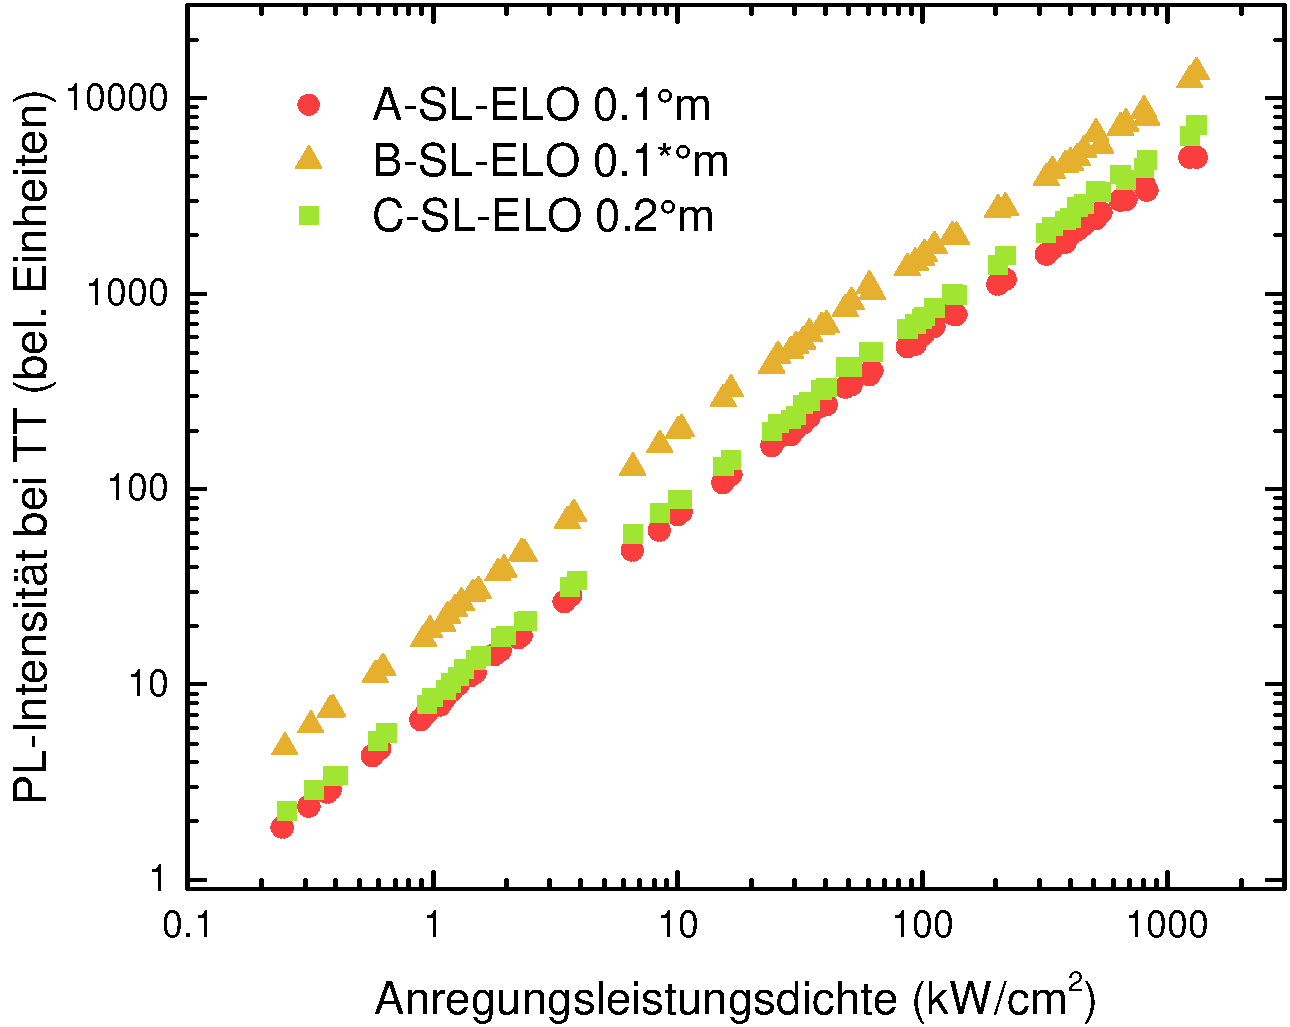
\includegraphics[width=\linewidth]{Bilder/TS4048/intTT.pdf}
		\caption{Die integrierte Intensität in Abhängigkeit der Anregungsleistungsdichte bei Tieftemperatur in doppelt-logarithmischer Darstellung.}
		\label{fig:sleloINTtt}
  \end{minipage}
\end{figure}
\noindent 
% 
Die integrierten Intensitäten in Abhängigkeit der Anregungsleistungsdichte (Abb. \ref{fig:intttrtsl}) zeigen, dass die Probe B-SL-ELO bei TT am stärksten leuchtet und bei Raumtemperatur auf gleichem Niveau mit der Probe A-SL-ELO ist. Die Probe C-SL-ELO leuchtet dagegen im Vergleich bei TT und RT am schwächsten, fällt allerdings nicht so signifikant gering gegenüber den anderen Proben aus, wie die Probe C-ELO aus der ersten Serie.
%
\begin{figure}[H]
  \centering
  \begin{minipage}[t]{0.49\textwidth}
    \centering
    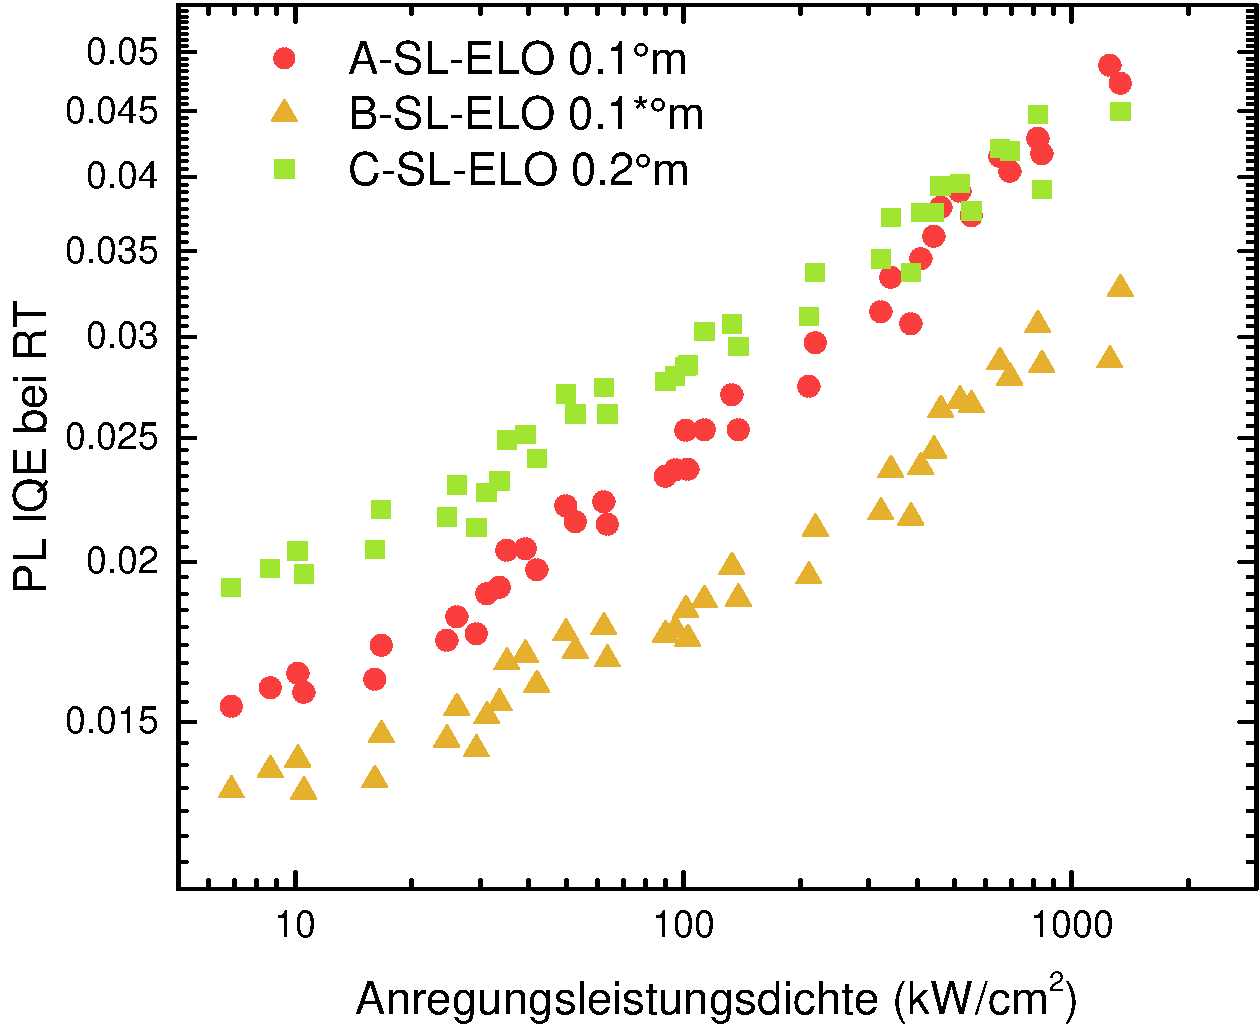
\includegraphics[width=\textwidth]{Bilder/TS4048/corrIQERT.pdf}
		\caption{Die IQEs für die Proben A-SL-ELO, B-SL-ELO und C-SL-ELO bei Raumtemperatur.}
    \label{fig:eloiqeRT}
  \end{minipage}
	\hfill
  \begin{minipage}[t]{0.49\textwidth}
    \centering
    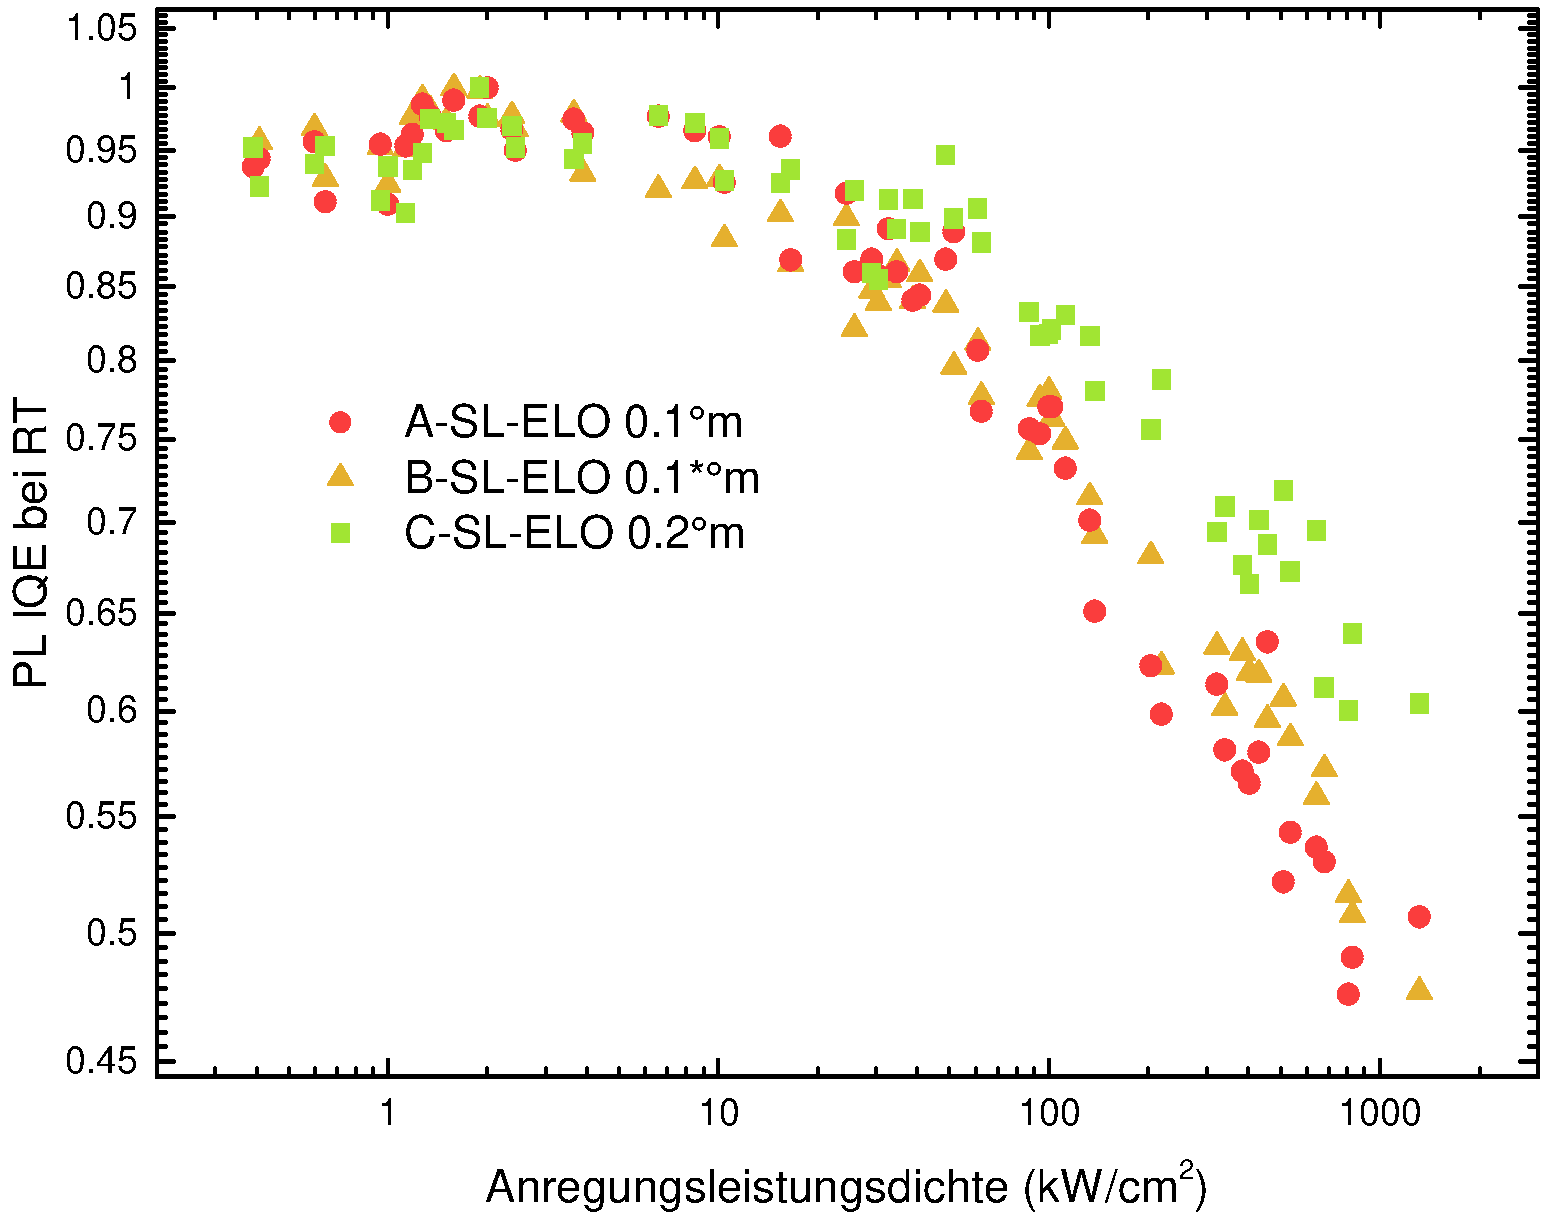
\includegraphics[width=\linewidth]{Bilder/TS4048/IQETT.pdf}
		\caption{Die IQEs für die Proben A-SL-ELO, B-SL-ELO und C-SL-ELO Tieftemperatur.}
    \label{fig:slelocorriqeRT}
  \end{minipage}
\end{figure}
\noindent 
%
Die IQEs der Proben bei RT und TT sind in Abbildung \ref{fig:eloiqeRT} und \ref{fig:slelocorriqeRT} zu sehen und zeigen, dass die Proben A-SL-ELO und C-SL-ELO die höchsten IQEs haben. Die Probe C-SL-ELO weist bei geringen Anregungsleistungsdichten die höchste IQE auf. A-SL-ELO weist in Abhängigkeit der Anregungsleistungsdichte die größte Steigung auf, sodass bei der höchsten Anregungsleistungsdichte bei $ 1300 \frac{kW}{cm^2} $ die IQEs beider Proben fast gleich sind mit $IQE_{A-SL-ELO} = 0,049 $ und $IQE_{C-SL-ELO} = 0,045$. C-SL-ELO fällt im Vergleich mit $IQE_{C-SL-ELO} = 0,033$ stark ab.  
%
\begin{figure}[H]
\begin{tabular}{ccc}
  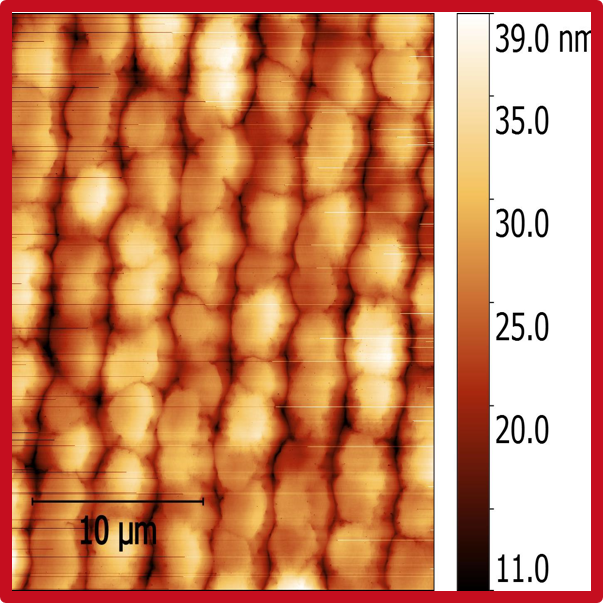
\includegraphics[width=0.30\textwidth]{Bilder/TS4048/aSLELOafm.png} & 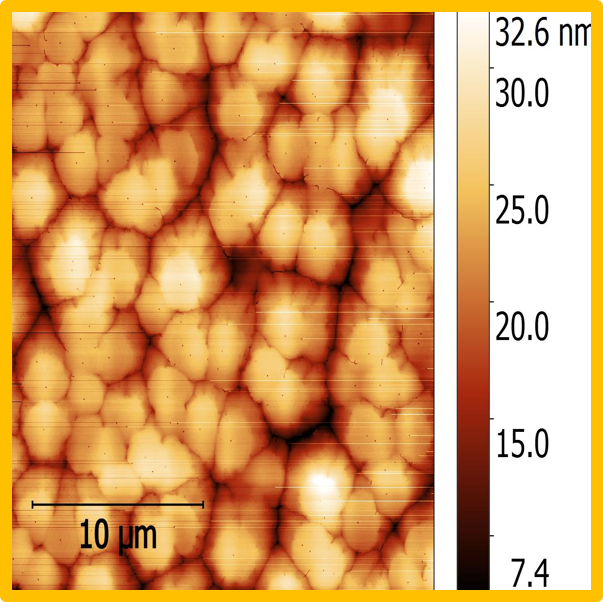
\includegraphics[width=0.30\textwidth]{Bilder/TS4048/bSLELOafm.png}  & 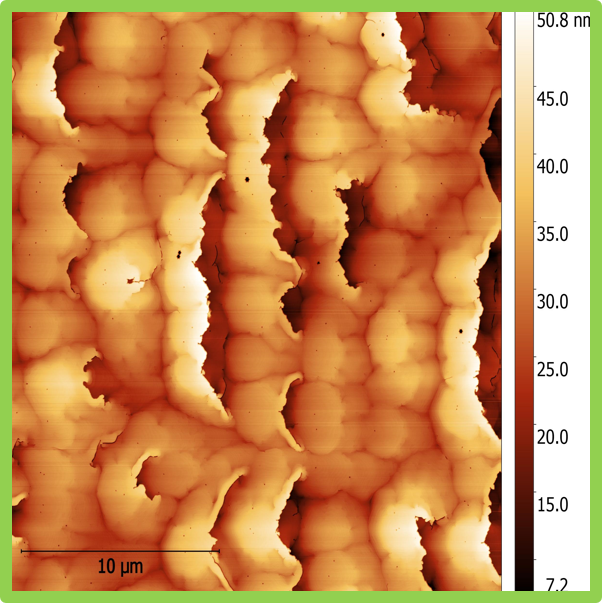
\includegraphics[width=0.30\textwidth]{Bilder/TS4048/cSLELOafm.png} \\
(a) & (b) & (c) \\[6pt]
 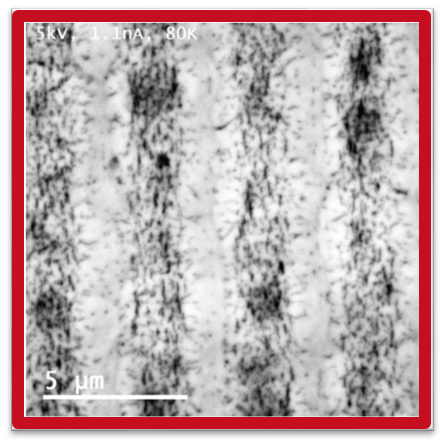
\includegraphics[width=0.30\textwidth]{Bilder/TS4048/aSLELOcl2.png} &   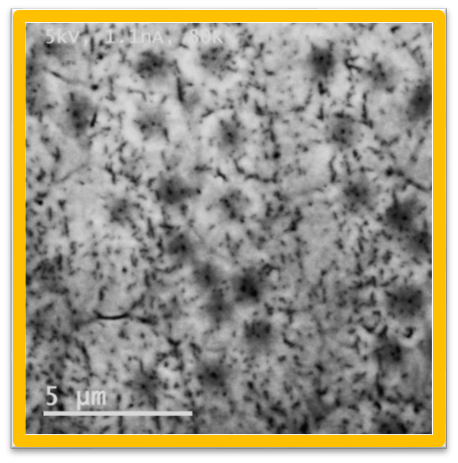
\includegraphics[width=0.30\textwidth]{Bilder/TS4048/bSLELOcl2.png} & 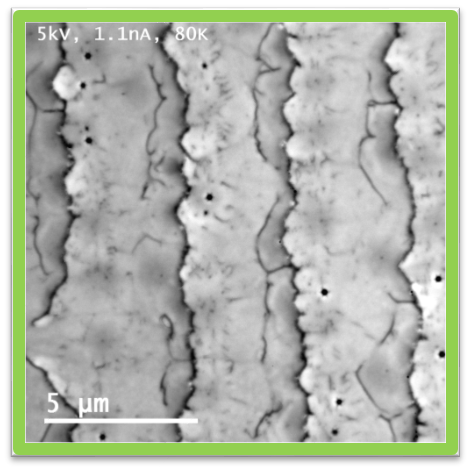
\includegraphics[width=0.30\textwidth]{Bilder/TS4048/cSLELOcl2.png}  \\
(d)  & (e) & (f)   \\[6pt]
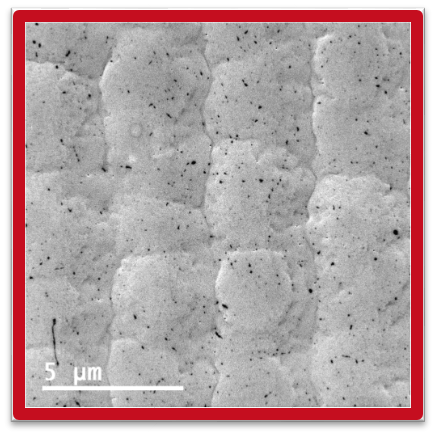
\includegraphics[width=0.30\textwidth]{Bilder/TS4048/aSLELOcl1.png} & 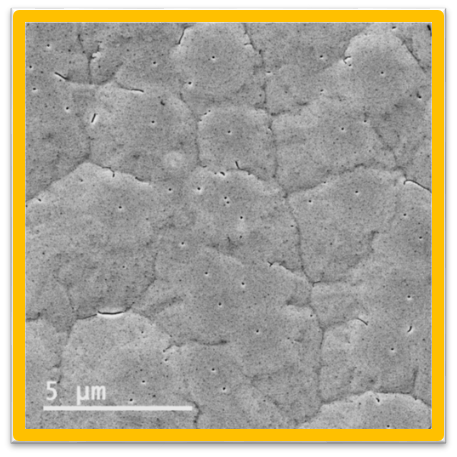
\includegraphics[width=0.30\textwidth]{Bilder/TS4048/bSLELOcl1.png}  & 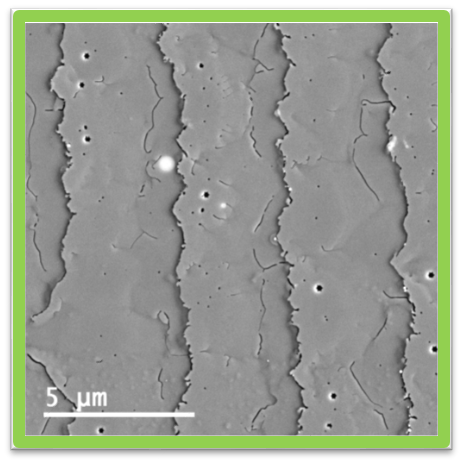
\includegraphics[width=0.30\textwidth]{Bilder/TS4048/cSLELOcl1.png} \\
(g)  & (h) & (i)   \\[6pt]
\end{tabular}
\caption{AFM-Bilder (a, b) und eine Limi-Aufnahme (c) von Christian Kuhn aufgenommen. SEM (c, d, e) und panchromatische CL-Aufnahmen(f, g, h) an den selben Stellen gemessen von Ute Zeimer (FBH)}
\label{fig:morph2}
\end{figure}
\noindent 
Hatten beide Proben mit dem selben Fehlschnittwinkel von $0,1 \degree$ in der ersten Serie noch nahezu die selben IQEs, weichen sie in dieser Serie deutlich von einander ab. Einen Grund dafür liefert möglicherweise die panchromatische-CL Aufnahme \ref{fig:morph2} (d) im Vergleich mit \ref{fig:morph1} (d). Dort ist erkennbar, dass die dunklen Punkte ebenfalls verteilt auf der Oberfläche zu sehen sind, jedoch in \ref{fig:morph2} (d) die Anzahl kleinerer dunkler Punkte um die kreisförmig angesammelten dunklen Punkte deutlich höher ist. Was auf eine höhere Anzahl an Defekten spricht und somit die geringe IQE erklären würde. Die AFM-Bilder in Abbildung \ref{fig:morph2} (a) (b) (c) zeigen eine ähnliche aber glattere Oberflächenmorphologie wie in der ersten Serie für die Proben mit dem selben Fehlschnittwinkel- und richtung. A-SL-ELO zeigt wie die A-ELO Spiralen entlang der ELO-Streifen auf dem AFM-Bild (a) und auf dem CL-Bild (d) sieht man ebenso dunkle Punkte hauptsächlich an den Kämmen der ELO-Streifen zwischen den geätzten Gräben. B-SL-ELO hat wie Probe B-ELO zufällig verteilte Spiralen auf der Oberfläche (b). Die SEM-Aufnahme (h) zeigt im Unterschied zur SEM-Aufnahme der Probe B-ELO Gruben im Zentrum der Wachstumsinseln. 
\begin{figure}[H]
  \centering
  \begin{minipage}[t]{0.49\textwidth}
    \centering
    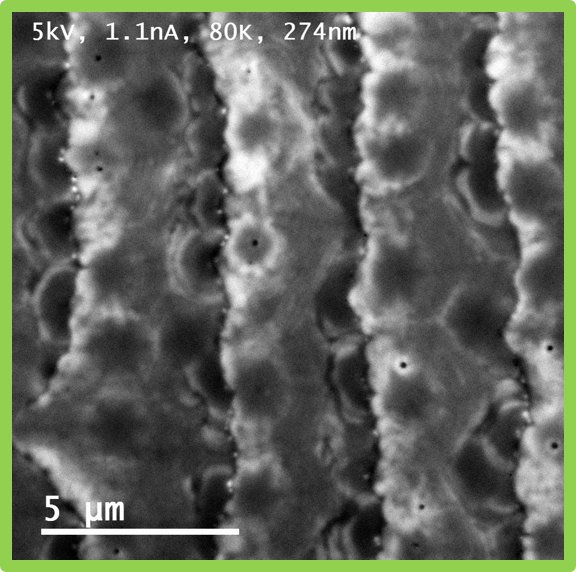
\includegraphics[width=0.7\textwidth]{Bilder/TS4048/cSLELOmonocllow.png}
		\caption{(a)}
  \end{minipage}
	\hfill
  \begin{minipage}[t]{0.49\textwidth}
    \centering
    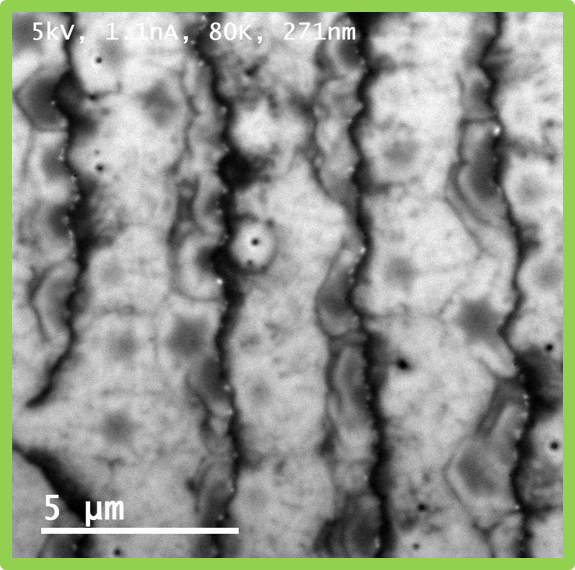
\includegraphics[width=0.7\linewidth]{Bilder/TS4048/cSLELOmonoclpeak.png}
		\caption{(b)}
  \end{minipage}
	\caption{Monochromatische CL-Bilder aufgenommen bei $80 \thinspace K$ bei $274 \thinspace nm$ und $271 \thinspace nm$. }
	\label{fig:monoclgesamt}
\end{figure}
\noindent 
Die Probe C-SL-ELO dagegen unterscheidet sich stark von C-ELO bezüglich der Oberflächenmorphologie, so tritt sporadisches Stufenbündelwachstum auf, was für einen Fehlschnitt von $0,14 \degree$, also nah an der Grenze von Stufenfluss- zu Stufenbündelwachstum spricht. Der Einbau von Gallium an den Stufenkanten bestätigt sich in den Mono-CL Aufnahmen bei $274 \thinspace nm$ und $271 \thinspace nm$(QW-Peak) bei TT ($80K$). So ist im Vergleich ersichtlich, dass Gallium an den Stufenkanten eingebaut wurde und zusätzlich sind noch pyramidenartige Strukturen mit Al-Gehalt zu sehen. Lokalisierungseffekte sind allerdings aufgrund der Diffusionslänge von ca. $100 \thinspace nm$ nicht zu erwarten. Aber auch hier scheint es, wie bei Probe C-ELO, Unterschiede in der Absorption der auf der Probe ankommenden Photonen zu geben, denn das Plateau der IQE bei TT beginnt bereits bei höheren Anregungsleistungsdichten im Vergleich zu A-SL-ELO und B-SL-ELO. Somit gilt auch hier, um den tatsächlichen Einfluss eines Fehlschnittwinkels von 0.2$^\circ$ auf die Defektdichte und damit auf die IQE zu bestimmen, wäre es notwendig eine maximale IQE zu bestimmen. Letzteres ist mit dem derzeitigen PL-Aufbau nicht möglich.


\section{Zusammenfassung}

\begin{figure}[H]
\centering
\begin{tabular}{ |c|c|c|c|c|c|   }
\hline
\multicolumn{3}{|c|}{Serie 1} & \multicolumn{3}{c|}{Serie 2}  \\
\hline
Name & Fehlschnittwinkel & IQE & Name & Fehlschnittwinkel & IQE \\
\hline
A-ELO & 0.1$^\circ$m & 0,055 & A-SL-ELO & 0.1$^\circ$m & 0,049  \\
B-ELO & 0.1$^\circ$m*& 0,054& B-SL-ELO & 0.1$^\circ$m* & 0,033 \\
C-ELO & 0.2$^\circ$m & 0,098& C-SL-ELO & 0.2$^\circ$m & 0,045 \\
\hline
\end{tabular}
\caption{IQEs beider Serien bei einer Anregungsleistungsdichte von $ 1300 \frac{kW}{cm^2} $.}
\end{figure}
\noindent 
Zusammenfassend lässt sich sagen, dass die Proben mit Übergitter eine eindeutig glattere Oberfläche aufweisen und damit einen wichtigen positiven Effekt für UVC-Laserdioden im Betrieb mit sich bringen. Die AFM-, SEM- und CL-Aufnahmen bestätigen, dass der Fehlschnittwinkel Einfluss auf die Wachstumskinetik hat. 
\noindent 
So ist in beiden Serien eindeutig der Einfluss der Fehlschnittrichtung zur Richtung der ELO-Streifen an der Oberflächenmorphologie zu erkennen. Auch Stufenbündelwachstum bei einem Fehlschnittwinkel von $0.2\degree$ hat sich bei Probe C-SL-ELO bestätigt. Ein positiver Einfluss auf die Defektdichte bei einem Fehlschnittwinkel von $0.2 \degree$ ist bei alleiniger Betrachtung der IQE der Probe C-ELO, bei der beim MQW-Wachstum etwas schief lief, zwar zu bestätigen, hat sich bei tiefergehender Analyse nicht erhärtet und gezeigt, dass es für eine verwertbare Analyse noch weiterer Investigation bedarf. 
\noindent 
Die Probe C-SL-ELO dagegen verhält sich ohne Widersprüche und zeigt eine der höchsten IQEs, die auf dem Niveau der A-ELO und A-SL-ELO ist. Bestätigt allerdings auch bei genauerer Betrachtung, dass für einen verwertbaren Vergleich, die Bestimmung einer maximalen IQE nötig ist, da für die Proben mit $0.2\degree$ offensichtlich andere Absorptionskoeffizienten gelten. 
\noindent 
C-SL-ELO weist eine rauere Oberfläche auf, weswegen für eine Verwendung in UVC-Laserdioden die Ergebnisse für die Verwendung von Übergittern mit einem Fehlschnitt von $0.1\degree$ sprechen
Dies bestätigt sich ebenfalls in den Untersuchungen von Christian Kuhn, die zeigen, dass mit Übergitter gewachsene UVC-Laser eine Reduktion der Laserschwelldichte um einen Faktor zwei im Vergleich zu ohne Übergitter gewachsene UVC-Laser aufweisen \cite{doi:10.1002/pssa.201870032}.